\documentclass[12pt]{report} % Times New Roman, 12pt
%\usepackage{gscale_thesis_singlespace} % Single spaced thesis
\usepackage{gscale_thesis_doublespace} % Double spaced thesis
\usepackage{fancyheadings} % Header and footer styling
\usepackage{natbib} % Bibliography formatting
\usepackage{setspace} % Allows double spacing but skips headers/footers
\setcounter{tocdepth}{2} % Limits the TOC to chapter and section names
\setcounter{chapter}{-1}

% Additional packages
\usepackage{graphicx} % Allows the inclusion of figures
\usepackage{subcaption} % Allows captions to be added to subfigures
\usepackage[justification=centering]{caption} % Centres caption text
\usepackage{array} % Used for table formatting
\newcolumntype{P}[1]{>{\raggedright\let\newline\\\arraybackslash\hspace{0pt}}m{#1}}
\usepackage{booktabs} % Fancy-style tables
\usepackage{longtable} % Allows for tables that are more than one page long
\usepackage{float} % Better figure placement control
\usepackage{enumerate} % Numbered lists
\usepackage[shortlabels]{enumitem} % For controlling enumerate labels
\usepackage[shortcuts]{extdash} % Allows manual hyphenation of hypenated words
\usepackage{amsmath} % Non-standard math symbols
\usepackage{amsfonts} % Extended fonts for mathematics
\usepackage[hidelinks]{hyperref} % Linking to LaTeX labels and external URLs
\hypersetup{
  colorlinks=true,
  linkcolor=black,
  filecolor=blue,      
  urlcolor=blue,
  citecolor=blue,
}
\usepackage{slashbox}
\usepackage{tikz}
\def\checkmark{\tikz\fill[scale=0.4](0,.35) -- (.25,0) -- (1,.7) -- (.25,.15) -- cycle;} 

\numberwithin{equation}{section} % Numbers equations based on their section

\usepackage[newfloat]{minted}
\newenvironment{code}{\captionsetup{type=listing}}{}
\SetupFloatingEnvironment{listing}{name=Code, listname=List of Codes}

\usepackage{tcolorbox} % Code section 
\tcbuselibrary{minted,skins}
\definecolor{bg}{rgb}{0.99, 0.96, 0.89}
\newtcblisting{haskell1}{
  listing engine=minted,
  colback=bg,
  colframe=black!70,
  listing only,
  minted style=colorful,
  minted language=haskell,
  minted options={linenos=true, texcl=true, breaklines=true, tabsize=2},
  left=1mm,
}
\newtcblisting{python1}{
  listing engine=minted,
  colback=bg,
  colframe=black!70,
  listing only,
  minted style=colorful,
  minted language=python,
  minted options={linenos=true, texcl=true, breaklines=true, tabsize=2},
  left=1mm,
}
\newtcblisting{java1}{
  listing engine=minted,
  colback=bg,
  colframe=black!70,
  listing only,
  minted style=colorful,
  minted language=csharp,
  minted options={linenos=true, texcl=true, breaklines=true, tabsize=2},
  left=1mm,
}
\newtcblisting{csharp1}{
  listing engine=minted,
  colback=bg,
  colframe=black!70,
  listing only,
  minted style=colorful,
  minted language=csharp,
  minted options={linenos=true, texcl=true, breaklines=true, tabsize=2},
  left=1mm,
}
\newtcblisting{cplusplus1}{
  listing engine=minted,
  colback=bg,
  colframe=black!70,
  listing only,
  minted style=colorful,
  minted language=csharp,
  minted options={linenos=true, texcl=true, breaklines=true, tabsize=2},
  left=1mm,
}

\usepackage{rotating} 
\usepackage{adjustbox}
\usepackage[mathletters]{ucs}
\usepackage[utf8x]{inputenc}

\newcommand{\highlight}[2]{\colorbox{#1}{$\displaystyle #2$}}

\usepackage{listings}
\usepackage{tocloft}

% ********************************
\begin{document}
\renewcommand\lstlistlistingname{List of Code}

\newcommand{\listequationsname}{List of Equations}
\newlistof{myequations}{equ}{\listequationsname}
\newcommand{\myequations}[1]{%
\addcontentsline{equ}{myequations}{\protect\numberline{\theequation}#1}\par}
\setlength{\cftmyequationsnumwidth}{2.5em}

\title{Generating Jupyter Notebooks in Drasil}
\halftitle{Generating Jupyter Notebooks in Drasil} % 60 Characters Max. 
%Including Spaces

\author{Ting-Yu Wu}
\shortauthor{Ting-Yu Wu} % Used for page header

\dept{Department of Computing and Software}
\field{Computing and Software} % What field your thesis is in (e.g. Software 
%Engineering)

\prevdegreeone{B.Sc. (Information \& Computer Engineering),\\Chung Yuan 
Christian University, Taoyuan, Taiwan}
\prevdegreetwo{B.Sc.} % Just your degree's field

\submitdate{April 2023} % Use the month's full spelling e.g. November
\copyrightyear{2023} % Year you are submitting this, usually your graduation 
%year

\doctype{Report} % ``Report'' or ``Thesis'' or whatever you need
\degree{Masters of Engineering} % The degree you get when you submit this
\degreeabbrv{M.Eng.}
\principaladviser{Dr. Spencer Smith and Dr. Jacques Carette} % Your Supervisor
 % LaTeX variables for preface pages/headers
    
\beforepreface % Half title page, title page, declaration page   
  % \prefacesection{Lay Abstract}

A lay abstract of not more 150 words must be included explaining the key goals and contributions of the thesis in lay terms that is accessible to the general public.  % Lay Abstract
  \prefacesection{Abstract}
Drasil is a framework that generates software, including code, documentation, software requirement specification, user manual, and axillary files. Recently, the Drasil team has been interested in expanding its knowledge to solve higher-order ODEs. In this research, for single higher-order linear ODEs, the Drasil framework can solve them without manually extracted information. For higher-order nonlinear ODEs, the Drasil framework can solve them with manually extracted information.

Firstly, we design a flexible and reusable structure to store ODE information based on conventional mathematical knowledge. This makes it possible to reuse ODE information for documentation and for code generation. Secondly, we provide a commonality analysis of four external ODE solver libraries. The analysis includes how they solve the ODE, what algorithms they use, and what options they provide for different types of output. Thirdly, we enable the Drasil Code Generator to solve nonlinear higher-order ODEs with some manually extracted information. We created a new case study, Double Pendulum, that has a system of higher-order ODE. Further, we solve the Double Pendulum example numerically via external libraries. Lastly, for single higher-order ODEs, the Drasil Code Generator can generate code without manually extracted information.

This research accomplishes three main goals. Firstly, we capture the knowledge of linear ODE in a flexible and reusable structure. Secondly, we expand the Drasil capability to solve higher-order ODEs with/without manually written equations. Solving single higher-order linear ODEs does not require manually extracted information. To solve nonlinear ODEs, manually extracting information from the original ODE is still required. The last one is removing the duplicated information caused by the implementation of solving ODEs. % Abstract
  % %\thispagestyle{empty}
\null\vfill
\begin{center}
%\textbf{Dedications}
%\linebreak
\textsl{Your Dedication \\ Optional second line}
\end{center}
\vfill
 % Dedication
  \prefacesection{Acknowledgements}

I would like to express my deepest appreciation to my supervisors, Dr.\ Spencer Smith and Dr.\ Jacques Carette. With their guideline, I could break a complex puzzle into smaller pieces and accomplish them one by one. I spent 90\% of my time in remote learning, but the quality of knowledge I received beyond learning in-person. My supervisors quickly adapted the work rhythm during the pandemic, and I greatly benefited from it.

Special thanks to my friend and colleague Jason Balaci for answering my questions and providing excellent suggestions for learning.

I am also thankful to my parents for supporting me in pursuing my second master's degree. Although my parents received very little education, they supported me in pursuing higher education mentally and financially.

Lastly, I want to thank Sophie for motivating me out of the bottom rock of my life.  % Acknowledgements
  \tableofcontents
  \listoffigures
  \pagebreak
  \listoftables
  \pagebreak
  \lstlistoflistings
  \pagebreak
  \listofmyequations
  % \referencepages % Table of Contents, List of Figures, List of Tables
  % \prefacesection{Notation, Definitions, and Abbreviations}
\ds{TODO: Update this}
\section*{Notation}
\begin{description}[font=\rmfamily\bfseries, leftmargin=3cm, style=nextline]
	\item[$A \leq B$] A is less than or equal to B
\end{description}

\section*{Definitions}
\begin{description}[font=\rmfamily\bfseries, leftmargin=3cm, style=nextline]
	\item[\SF] A portmanteau of `software' and `artifact'. The term refers to 
	any of the artifacts (documentation, code, test cases, build instructions, 
	etc.) created during a software project's development.
\end{description}

\section*{Abbreviations}
\begin{description}[font=\rmfamily\bfseries, leftmargin=3cm, style=nextline]
	\item[QA] Quality Assurance
	\item[SI] Syst\`eme International d'Unit\'es
	\item[SRS] Software Requirements Specification
\end{description}
  \lastpageofpreface{notation}
\afterpreface
  
  \chapter{Background}
\section{Software Artifacts}
\label{sec:sfs}

Software artifacts (or \sfs{}) come in a wide variety of forms and have existed 
since the first programs were created. In the broadest sense, we can think of 
\sfs{} as anything produced during the creation of a piece of software that 
serves some purpose. Any document detailing what the software should do, how it 
was designed, how it was implemented, how to test it, and so on would be 
considered a \sf{}, as would the source code whether as a text file, stack of 
punched cards, magnetic tapes, or other media.

\ds{Need to work in (here?) why \sfs{} are important}

\fig{
\begin{center}
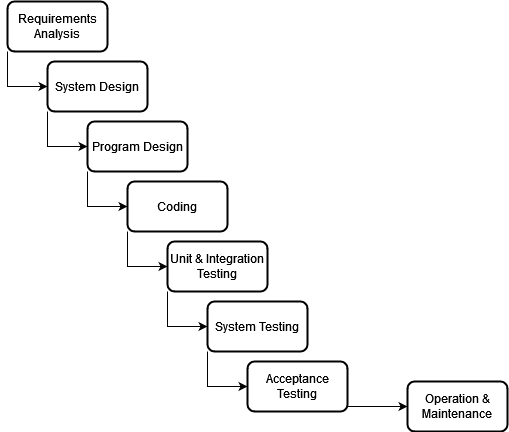
\includegraphics[width=\linewidth]{figures/Waterfall.png}
\end{center}}
{The Waterfall Model of Software Development}
{fig:Waterfall}

Software design can follow a number of different design processes, each with 
their own collection of \sfs{}. A common, traditional approach is the Waterfall 
model (Figure~\ref{fig:Waterfall}) of software 
development~\cite{PfleegerAndAtlee2010Ch2}. 
However, Parnas and Clements~\cite{ParnasAndClements1986} detailed what they 
dubbed a ``rational" design process; an idealized version of software 
development which includes what needs to be documented in corresponding \sfs{}.
The rational design process is not meant to be a linear process like the 
Waterfall model, but instead an iterative process using section stubs for 
information that is not yet available or not fully clear during the time of 
writing. Those stubs are then filled in over the development process, and 
existing documentation is updated so it appears to have been created in a 
linear fashion for ease of review later in the software lifecycle. The rational 
design process involves the following:

\begin{enumerate}
\item Establish/Document Requirements
\item Design and Document the Module Structure
\item Design and Document the Module Interfaces
\item Design and Document the Module Internal Structures
\item Write Programs
\item Maintain
\end{enumerate}

Parnas provided a list of the most important documents~\cite{Parnas2010} 
required for the rational design process, which Smith~\cite{Smith2016} 
\ds{which paper was it?} expanded upon by including complimentary artifacts 
such as source code, verification and validation plans, test cases, and build 
instructions. While there have been many proposed artifacts, the following 
curated list covers those most relevant to this thesis:

\begin{enumerate}
\item System Requirements
\item System Design Document
\item Module Guide
\item Module Interface Specification
\item Program Source Code
\item Verification and Validation Plan
\item Test cases
\item Verification and Validation Report
\item User Manual
\end{enumerate}

This list is not exhaustive of all the types of \sfs{}, as there are many other
design processes which use different types of \sfs{}. Looking at an agile 
approach using Scrum/Kanban, the \sfs{} tend to be distributed in different 
ways. Requirements are documented in tickets under so-called `epics', 
`stories', and `tasks' as opposed to a singular requirements artifact, and the 
acceptance criteria listed on those tickets make up the validation and 
verification plan. 

Regardless of the process used, most attempt to document very similar 
information to that of the rational design process. Using the waterfall model 
as an example, we can see (Table~\ref{tab:RatWatComp}) the rational design 
process and its artifacts map onto the model in a very straightforward manner.

\begin{table}[htbp]
\caption{Comparison of Rational Design Process and Waterfall Model}
\label{tab:RatWatComp}
\begin{tabular}{|p{.25\linewidth}|p{.35\linewidth}|p{.4\linewidth}|}
\hline &&\\
Rational Design phase & Corresponding Waterfall phase(s) & Common \SFS{}
\\&&\\ \hline &&\\
	Establish/ Document Requirements & Requirements Analysis & System 
	Requirements Specification \newline \newline
	Verification and Validation plan
\\&&\\ \hline &&\\
	Design and Document the Module Structure & 
	System Design  & 
	Design Document
\\&&\\ \hline &&\\
	Design and Document the Module Interfaces & 
	Program Design & 
	Module Interface Specification
\\&&\\ \hline &&\\
	Design and Document the Module Internal Structures &
	Program Design &
	Module Guide
\\&&\\ \hline &&\\
	Write Programs & 
	Coding &
	Source code  \newline \newline
	Build instructions
\\&&\\ \hline &&\\
	Maintain & 
	Unit \& Integration Testing \newline \newline System Testing \newline 
	\newline Acceptance 
	Testing \newline \newline Operation \& Maintenance &
	Test cases \newline \newline
	Verification and Validation Report
\\ \hline
\end{tabular}
\end{table}

\SFS{} are important to development in a number of ways, such as easing the 
burden of maintenance and training. We outline the artifacts we are most 
interested below with a brief description of their purpose.

\cardifact{Software Requirements Specification}{Contains the functional and 
nonfunctional requirements detailing what the desired software system should 
do.}
\cardifact{System Design Document}{Explains how the system should be broken 
down and documents implementation-level decisions that have been made for the 
design of the system.}
\cardifact{Module Guide}{In-depth explanation of the modules outlined in the 
System Design Document.}
\cardifact{Module Interface Specification}{Interface specification for each of 
the modules outlined in the System Design Document/Module Guide.}
\cardifact{Program Source Code}{The source code of the implemented software 
system.}
\cardifact{Verification and Validation Plan}{Uses the system requirements to 
document acceptance criteria for each requirement that can be validated.}
\cardifact{Test cases}{Implementation of the Verification and Validation Plan 
in source code (where applicable) or as a step-by-step guide for testers.}
\cardifact{Verification and Validation Report}{Report outlining the results 
after undertaking all of the testing initiatives outlined in the Verification 
and Validation plan and test cases.}

\section{Software Reuse and Software Families}
\subsection{Software/Program Families}
  - Bring up GNU/Linux and different distros as examples of software families
    - (Raspbian v Raspbian lite) = Debian--, etc.
\subsection{Reuse and Reproducible Research}
  - Touch on reuse areas like reproducible research - Gentleman and Lang 2012

Being able to reproduce results, is fundamental to the idea of good science.
When it comes to software projects, there are often many undocumented
assumptions or modifications (including hacks) involved in the finished product.
This can make replication impossible without the help of the original author,
and in some cases reveal errors in the original author's
work~\cite{IonescuAndJansson2013}.

Reproducible research has been used to mean embedding executable code in
research papers to allow readers to reproduce the results
described~\cite{SchulteEtAl2012}.

Combining research reports with relevant code, data, etc.\ is not necessarily
easy, especially when dealing with the publication versions of an author's work.
As such, the idea of \emph{compendia} were
introduced~\cite{GentlemanAndLang2012} to provide a means of encapsulating the
full scope of the work. Compendia allow readers to see computational details, as
well as re-run computations performed by the author. Gentleman and Lang proposed
that compendia should be used for peer review and distribution of scientific
work~\cite{GentlemanAndLang2012}.

Currently, several tools have been developed for reproducible research
including, but not limited to, Sweave~\cite{Leisch2002},
SASweave~\cite{LenthEtAl2007}, Statweave~\cite{Lenth2009},
Scribble~\cite{FlattEtAl2009}, and Org-mode~\cite{SchulteEtAl2012}. The most
popular of those being Sweave~\cite{SchulteEtAl2012}. The aforementioned tools
maintain a focus on code and certain computational details. Sweave,
specifically, allows for embedding code into a document which is run as the
document is being typeset so that up to date results are always included.
However, Sweave (along with many other tools), still maintains a focus on
producing a single, linear document. It is my hope that Drasil will outperform
these existing tools due to its flexibility and its ability to create multiple
artifacts from a knowledge base.

\section{Literate Approaches to Software Development}

There have been several approaches attempting to combine development of program 
code with documentation. Literate Programming and literate software are two 
such approaches that have influenced the direction of this thesis. Each of 
these approaches is outlined in the following sections.

\subsection{Literate Programming}

Literate Programming (LP) is a method for writing software introduced by Knuth 
that focuses on explaining to a human what we want a computer to do rather than 
simply writing a set of instructions for the computer on how to perform the 
task~\cite{Knuth1984}.

Developing literate programs involves breaking algorithms down into
\emph{chunks}~\cite{JohnsonAndJohnson1997} or \emph{sections}~\cite{Knuth1984}
which are small and easily understandable. The chunks are ordered to follow a 
``psychological order''~\cite{PieterseKourieAndBoake2004} if
you will, that promotes understanding. They do not have to be written in the 
same order that a computer would read them. It should also be noted that in a 
literate program, the code and documentation are kept together in one source. 
To extract runnable code, a process known as \emph{tangle} must be performed on 
the source. A similar process known as \emph{weave} is used to extract and 
typeset the documentation.

There are many advantages to LP beyond understandability. As a program is
developed and updated, the documentation surrounding the source code is more 
likely to be updated simultaneously. It has been experimentally found that 
using LP ends up with more consistent documentation and 
code~\cite{ShumAndCook1993}. There are many downsides to having inconsistent 
documentation while developing or maintaining 
code~\cite{Kotula2000,Thimbleby1986}, while the benefits of consistent 
documentation are numerous~\cite{Hyman1990, Kotula2000}. Keeping the advantages 
and disadvantages of good documentation in mind we can see that more effective, 
maintainable code can be produced if properly using 
LP~\cite{PieterseKourieAndBoake2004}.

Regardless of the benefits of LP, it has not been very popular with 
developers~\cite{ShumAndCook1993}. However, there are
several successful examples of LP's use in SC. Two such literate programs that 
come to mind are VNODE-LP~\cite{Nedialkov2006} and ``Physically Based 
Rendering: From Theory to Implementation''~\cite{PharrAndHumphreys2004} a 
literate program and textbook on the subject matter. Shum and 
Cook~\cite{ShumAndCook1993} discuss the main issues behind LP's lack of 
popularity which can be summed up as dependency on a 
particular output language or text processor, and the lack of flexibility on 
what should be presented or suppressed in the output.

There are several other factors which contribute to LP's lack of popularity and 
slow adoption thus far. While LP allows a developer to write their code and its 
documentation simultaneously, that documentation is comprised of a single 
artifact which may not cover the same material as standard artifacts software 
engineers expect (see Section~\ref{sec:sfs} for more details). LP also does not 
simplify the development process: documentation and code are written as usual, 
and there is the additional effort of re-ordering the chunks. The LP 
development process has some benefits such as allowing developers to follow a 
more natural flow in development by writing chunks in whichever order they 
wish, keep the documentation and code updated simultaneously (in theory) 
because of their co-location, and automatically incorporate code chunks into 
the documentation to reduce some information duplication.

There have been many attempts to increase LP's popularity by focusing on 
changing the output language or removing the text processor dependency. Several
new tools such as CWeb (for the C language), DOC++ (for C++), noweb 
(programming language independent), and others were developed. Other tools such 
as javadoc (for Java) and Doxygen (for multiple languages) were also influenced 
by LP, but differ in that they are merely document extraction tools. They do 
not contain the chunking features which allow for re-ordering algorithms.

With new tools came new features including, but not limited to, phantom
abstracting~\cite{ShumAndCook1993}, a ``What You See Is What You Get'' (WYSIWYG)
editor~\cite{FritzsonGunnarssonAndJirstrand2002}, and even movement away from 
the ``one source'' idea~\cite{Simonis2003}.

While LP is still not mainstream~\cite{Ramsey1994}, these more robust 
tools helped drive the understanding behind what exactly LP tools must 
do. In certain domains LP is becoming more standardized, for 
example: Agda, Haskell, and R support LP to some extent, even though it is not 
yet common practice. R has good tool support, with the most popular being
Sweave~\cite{Leisch2002}, however it is designed to dynamically create
up-to-date reports or manuals by running embedded code as opposed to being used
as part of the software development process. 

\subsection{Literate Software}

A combination of LP and Box Structure~\cite{Mills1986} was proposed as a new
method called ``Literate Software Development''
(LSD)~\cite{AlMatiiAndBoujarwah2002}. Box structure can be summarized as the
idea of different views which are abstractions that communicate the same
information in different levels of detail, for different purposes. Box
structures consist of black box, state machine, and clear box structures. The
black box gives an external (user) view of the system and consists of stimuli
and responses; the state machine makes the state data of the system visible (it
defines the data stored between stimuli); and the clear box gives an internal
(designer's) view describing how data are processed, typically referring to
smaller black boxes~\cite{Mills1986}. These three structures can be nested as
many times as necessary to describe a system.

LSD was developed with the intent to overcome the disadvantages of both LP and
box structure. It was intended to overcome LP's inability to specify interfaces
between modules, the inability to decompose boxes and implement the design
created by box structures, as well as the lack of tools to support box
structure~\cite{Deck1996}.

The framework developed for LSD, ``WebBox'', expanded LP and box structures in a
variety of ways. It included new chunk types, the ability to refine chunks, the
ability to specify interfaces and communication between boxes, and the ability
to decompose boxes at any level. However, literate software (and LSD) remains
primarily code-focused with very little support for creating other software
artifacts, in much the same way as LP.

\section{Generative Programming}
 - ?
                  
    \setcounter{figure}{0}
    \setcounter{equation}{0}
    \setcounter{table}{0}

  \chapter{Introduction}
\ds{Introduce the term softifact somewhere in here}

\ds{Pain points and problems come first, then solution is docs, then problems 
with writing docs, then the rest of this.}
Documentation is good\citep{??}, yet it is not often prioritized on software
projects. Code and other software artifacts say the same thing, but to different
audiences - if they didn't, they would be describing different systems.

Take, for example, a software requirements document. It is a human-readable
abstraction of *what* the software is supposed to do. Whereas a design document
is a human-readable version of *how* the software is supposed to fulfill its
requirements. The source code itself is a computer-readable list of instructions
combining *what* must be done and, in many languages, *how* that is to be
accomplished.

[Put in figures of an example from GlassBR/Projectile here, showing SRS, DD, and
code versions of the same knowledge]

[Figure] shows an example of the same information represented in several
different views (requirements, detailed design, and source code). We aim to
take advantage of the inherent redundancy across these views to distill a single
source of information, thus removing the need to manually duplicate information
across software artifacts.

Manually writing and maintaining a full range of software artifacts (i.e.
multiple documents for different audiences plus the source code) is
redundant and tedious. Factor in deadlines, changing requirements, and other
common issues faced during development and you have a perfect storm for
inter-artifact syncronization issues.

How can we avoid having our artifacts fall out of sync with each other?
Some would argue "just write code!" And that is exactly what a number of other
approaches have tried. Documentation generators like Doxygen, Javadoc, Pandoc,
and more take a code-centric view of the problem. Typically, they work by having
natural-language descriptions and/or explanations written as specially delimited
comments in the code which are later automatically compiled into a
human-readable document.

While these approaches definitely have their place and can come in quite handy,
they do not solve the underlying redundancy problem. The developers are still
forced to manually write descriptions of systems in both code and comments.
They also do not generate all software artifacts - commonly they are used to
generate only API documentation targeted towards developers or user manuals.

We propose a new framework, Drasil, alongside a knowledge-centric view of
software, to help take advantage of inherent redundancy, while avoiding manual
duplication and synchronization problems. Our approach looks at what underlies
the problems we solve using software and capturing that "common" or "core"
knowledge. We then use that knowledge to generate our software artifacts, thus
gaining the benefits inherent to the generation process: lack of manual
duplication, one source to maintain, and 'free' traceability of information.

\section{Value in the mundane}
??

\section{Scope}
We are well aware of the ambitious nature of attempting to solve the problem of
manual duplication and unnecessary redundancy across all possible software
systems. Frankly, it would be highly impractical to attempt to solve such a
broad spectrum of problems. Each software domain poses its own challenges,
alongside specific benefits and drawbacks. 

Our work on Drasil is most relevant to software that is well-understood and 
undergoes frequent change (maintenance). Good candidates for development using
Drasil are long-lived (10+ years) software projects with artifacts of interest
to multiple stakeholders. With that in mind, we have decided to focus on
scientific computing (SC) software. Specifically, we are looking at software 
that follows the pattern 'input -> process -> output'.

SC software has a strong fundamental underpinning of well-understood concepts.
It also has the benefit of seldomly changing, and when it does, existing models
are not necessarily invalidated. For example, rigid-body problems in physics are
well-understood and the underlying modeling equations are unlikely to change.
However, should they change, the current models will likely remain as good
approximations under a specific set of assumptions. For instance, who hasn't
heard 'assume each body is a sphere' during a physics lecture?

\section{Roadmap}

\section{Contributions \& Publications}

\ds{After so much time working here, I think I've finally realized one of the 
true contributions of this thesis/Drasil. Not only the framework itself 
(which is still awesome), but also the process of breaking everything down and 
truly understanding softifacts at a deep level to operationalize our 
understanding of SE / system design in a way that makes all of this generation 
possible. With that in mind Drasil is just one means to that end.}

\ds{Minor point that came up in conversation: Parnas' paper on how/why to fake 
rational design. Our tool lets people fake it. It's all about change, there's 
no perfect understanding at the beginning and we need to change things on as we 
go. Drasil allows us to change everything to fake the rational design process 
at every step along the way.}

\ds{Continuous integration / refactoring are nothing new, but the way we used 
them ensured we were always at a steady-state where everything worked.}

\ds{Note that some of the code may not have been written by me directly, but 
was developed by the Drasil team}
                  
    \setcounter{figure}{0}
    \setcounter{equation}{0}
    \setcounter{table}{0}

  \chapter{ODE Data Representation}
In the Drasil framework, there is a single data structure containing all the information for all products; we call it \verb|System Information|. The giant \verb|System Information| collects a multitude of information; whenever we need it, we extract the information from \verb|System Information|. We store the ODE information in \verb|System Information|. 

An ODE can exist in various forms, with different forms suitable for different purposes. For example, we can transform a higher-order ODE into its equivalent system of first-order ODEs. The higher-order form is suitable for presenting the physics, but the system form is suitable for solving the ODE numerically. In previous research, we stored the ODE information in a data structure that cannot be reused for other purposes. We have to manually create the ODE in a specific form to satisfy a new goal each time. This is problematic because duplication cause problems for maintainability and traceability. In many projects, developers want to remove manually created code as much as possible because they are tedious and error-prone. For example, the \href{https://fenicsproject.org/}{FEniCS} is a project for solving differential equations. While solving differential equations with the finite element method, two variables, $A_T$ and $l_T$, are needed and usually calculated by hand (227)~\citep{loggetal2012}. To avoid creating special-purpose code, FEniCS developers decided to solve the problem by creating a form complier. Another example is the \href{https://math-atlas.sourceforge.net/}{ATLAS} project, a software tool for solving linear algebra. Researchers can implement many optimizations on specific platforms, but those optimizations may cause a slowdown on other platforms (3)~\citep{whaleyetal2001}. A traditional way of handling this problem is manually creating code for each platform. To avoid creating manually created code, ATLAS researchers decided to create a new paradigm called Automated Empirical Optimization. The Drasil team faces a similar problem: we manually extract necessary information from the original ODE. One solution is to explore a new way to store ODEs in a new data structure. The new structure must allow the different forms to be isomorphic, which means we can map one ODE form to another.

By capturing the essential information of ODEs, we can flexibly transform it into others forms that might appear. On the one hand, the transformation might result in losing information. For example, we can display an ODE in a textual form in the SRS (software requirements specification). Once we complete the transformation for displaying purposes, the textual form ODE has less information than the original ODE. On the other hand, we may make a transformation for a specific purpose, such as generating code for an ODE solver. Furthermore, capturing an ODE's information in a flexible data structure only requires a Drasil user to write the ODE's information once.

In this chapter, we will first introduce how we can rewrite ODE for a different purpose. Then, we will introduce a new data structure for storing ODE information. We will talk about details on how the new data structure captures ODE information, how to use the new data structure, and how the new data structure interacts with the Drasil Printer.

\section{Explicit Equation}
Before we conducted this project, the Drasil framework can generate software that provides numerical solutions for a first-order ODE by explicitly rewriting the ODE equation. We will rewrite the original ODE in a form which the Drasil Code Generator can utilize. The Drasil Code Generator retrieves ODE information from the new ODE form and generates a program that can produce numerical solutions. We will illustrate our steps with the \href{https://jacquescarette.github.io/Drasil/examples/nopcm/SRS/srs/NoPCM_SRS.html#Sec:IMs}{NoPCM case study}. Figure~\ref{fig_nopcm} shows how a NoPCM example works in a lab environment.
\begin{figure}[ht]
\centering
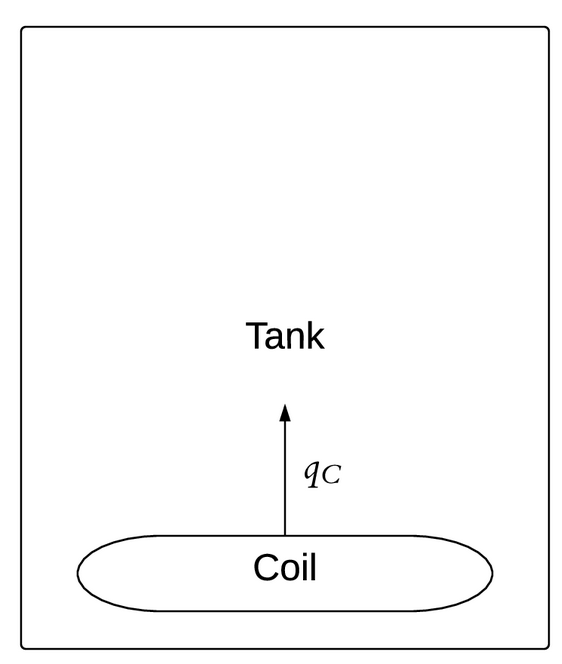
\includegraphics[width=0.3\textwidth]{figures/NoPCM.png}
\caption{NoPCM Demonstration}
\label{fig_nopcm}
\end{figure}
The rectangle represents a water tank, and it has a heating coil at the bottom of the tank. $qc$ represents the heat flux into the water from the coil. The goal is to estimate the temperature of the water over time. We can describe this natural phenomenon in a second-order ODE, Equation~\ref{eq_nopcmorginal}.

\begin{equation} \label{eq_nopcmorginal}
	T_{w}'(t) +  \frac {T_{w}(t)}{\tau_{w}} = \frac{T_{c}}{\tau_{w}}
\end{equation}
\myequations{NoPCM Equation}

$T_w(t)$ is a function of the independent variable, in this case time (t). $T_w$ is the temperature of water ($ ^\circ C $). $T_w'(t)$ is the first derivative of the function $T_w(t)$ with respect to time. $T_c$ is the temperature of the heating coil (°C), and $\tau_w$ is the ODE parameter for water related to decay time (s). Isolating for $T_w'(t)$, we obtain the following equation:
\begin{equation} \label{eq_nopcmderive}
	% T_{w}'(t) = \frac{T_{c} - T_{w}(t)}{\tau_{w}}
	T_{w}'(t) = \frac{1}{\tau_{w}} (T_{c} - T_{w}(t))
\end{equation}

\begin{listing}[ht]
\begin{haskell1}
-- Pseudocode for the readability
T_w'(t) = reciprocal τ_w * (T_c - T_w(t))
\end{haskell1}
\captionof{listing}{NoPCM Equation for SRS}
\label{code_expliciteqsrs}
\end{listing}

Based on Equation~\ref{eq_nopcmderive}, we can encode the syntax of the ODE in Code~\ref{code_expliciteqsrs} with the Drasil language. Although it has a basic mathematical structure, it is too hard-coded to make a transformation. We can use the information of Code~\ref{code_expliciteqsrs} for a display purpose, such as displaying the ODE equation in the SRS, because this form follows the syntax of the equation. However, we cannot reuse it for other purposes, such as creating a program that solves the ODE numerically. Therefore, we rewrite the Code~\ref{code_expliciteqsrs} to other forms for the purpose of solving the ODE. Brooks's thesis (91-103)~\citep{brooks} documented how the Drasil framework solves Equation~\ref{eq_nopcmderive} with the manually created \href{https://jacquescarette.github.io/Drasil/docs/drasil-code-0.1.9.0/Language-Drasil-Code.html#t:ODEInfo}{ODEInfo}. The \verb|ODEInfo| is a \verb|data type| that includes the necessary information from the original ODE (Equation~\ref{eq_nopcmderive}). The Drasil Code Generator can utilize \verb|ODEInfo| to generate a program that solves the original ODE numerically. 
\begin{listing}[ht]
\begin{haskell1}
-- Pseudocode for the readability
reciprocal τ_w * (T_c - T_w[0])
\end{haskell1}
\captionof{listing}{NoPCM Equation for the Drasil Code Generator}
\label{code_expliciteq}
\end{listing}
Code~\ref{code_expliciteq} shows how to rewrite the original ODE for the purpose of solving it. We cannot directly transform Code~\ref{code_expliciteqsrs} to Code~\ref{code_expliciteq}; there is a gap between two ODE expressions. $T\_w(t)$ is just a variable, but $T\_w[0]$ means the index of $0$ in $T\_w$. This assumes $T\_w$ is a list.

Despite the gap between Code~\ref{code_expliciteqsrs} and Code~\ref{code_expliciteq}, we can manually close it by rewriting the ODE. Rewriting the ODE in another form produces duplication because both Code~\ref{code_expliciteqsrs} and Code~\ref{code_expliciteq} describe the same ODE. The Code~\ref{code_expliciteqsrs} lacks the necessary structure to allow transformation. Therefore, we propose a new data structure to store the ODE information.

\section{Matrix Form Structure}
In general, an equation contains a left-hand expression, a right-hand expression, and an equal sign. The left-hand and right-hand expressions connect by an equal sign. A linear ODE also has its left-hand and right-hand sides. Each side has its unique shape. We can write a linear ODE in the shape of
\begin{equation} \label{eq_matrixform}
	\boldsymbol{Ax} = \boldsymbol{b}
\end{equation}
\myequations{Matrix Form}

On the left-hand side, $\boldsymbol{A}$ is an $m \times n$ matrix, and $\boldsymbol{x}$ is an $n$-vector. On the right-hand side, $\boldsymbol{b}$ is an $m$-vector. $\boldsymbol{A}$ is commonly known as the coefficient matrix, $\boldsymbol{x}$ is the unknown vector, and $\boldsymbol{b}$ is the constant vector. Equation~\ref{eq_matrixform} can represent not only a single linear ODE but also a linear system of ODEs. A linear system of ODEs is a finite set of linear differential equations. In this research, we have two case studies, NoPCM and PDController, for single higher-order linear ODEs and Double Pendulum for a system of higher-order nonlinear ODEs. The new data structure will be applied to single higher-order linear ODEs. This data structure is capable of storing information for a system of ODEs, but its related functions only support the case studies with a single ODE. Here is an ODE example from the \href{https://jacquescarette.github.io/Drasil/examples/pdcontroller/SRS/srs/PDController_SRS.html#Sec:IMs}{PDContoller case study}.
\begin{equation} \label{eq_odeexmaple}
	y''(t) + (1 + K_d) \cdot y'(t) + (20 + K_p) \cdot y(t) = r_t \cdot K_p
\end{equation}
\myequations{PDContoller Equation}

In Equation~\ref{eq_odeexmaple}, there is only one dependent variable $y$. The dependent variable $y$ is dependent on the independent variable $t$, in this case time. We use $y$(t) to represent a function of time. $y'$(t) is the first derivative of $y$(t). $y''$(t) is the second derivative of $y$(t). $y$ is the process variable, and $y'(t)$ is the rate of change of $y(t)$. $y''(t)$ is the rate of change of the rate of change of $y(t)$. $K_d$, $K_p$, and $r_t$ are constant variables. $K_d$ is Derivative Gain, $K_p$ is Proportional Gain, and $r_t$ is the Set-Point. We can write Equation~\ref{eq_odeexmaple} in a matrix form as follows:

\begin{equation} \label{eq_matrixformexmaple}
	\begin{bmatrix}
		1, & 1 + K_{d}, & 20 + K_{p}
	\end{bmatrix}
	\cdot
	\begin{bmatrix}
		y''(t)  \\
		y'(t)   \\
		y(t)  
	\end{bmatrix}
	=
	\begin{bmatrix}
		r_{t} \cdot K_{p} 
	\end{bmatrix}
\end{equation}
\myequations{PDContoller Equation in Matrix Form}

The relationship between the matrix form~\ref{eq_matrixform} and the Equation~\ref{eq_matrixformexmaple} is not hard to find. Firstly, the coefficient matrix $\boldsymbol{A}$ is a 1 $\times$ 3 matrix that consists of $1$, $1 + K_d$, ane $20 + K_p$. Secondly, the unknown vector $\boldsymbol{x}$ is a 3 $\times$ 1 vector with $y''(t)$, $y'(t)$, and $y(t)$. Lastly, the constant vector $\boldsymbol{b}$ is a 1 $\times$ 1 vector with $r_t \cdot K_p$. The matrix form~\ref{eq_matrixform} captures all the knowledge we need to present an ODE. However, what is the matrix form for a $n$th-order linear ODE? Based on Paul's Online Notes~\citep{paullinearode}, we can write all linear ODEs in the shape of

\begin{equation} \label{eq_linearDE}
	a_n(t) \cdot y^n(t) + a_{n-1}(t) \cdot y^{n-1}(t) + \dots + a_1(t) \cdot y'(t) + a_0(t) \cdot y(t) = h(t)
\end{equation}
\myequations{Linear Higher-Order ODE}

The coefficient $a_0(t), \dots, a_n(t)$ and $g(t)$ can be constant or non-constant functions, in our case they are constant functions. We also can write Equation~\ref{eq_linearDE} in a matrix form as
\begin{equation} \label{eq_matrixnthorder}
	\begin{bmatrix}
		a_n(t), & a_{n-1}, \dots, & a_0(t)
	\end{bmatrix}
	\cdot
	\begin{bmatrix}
		y^{n}(t) \\
		y^{n-1}(t) \\
		\dots \\
		y(t)  
	\end{bmatrix}
	=
	\begin{bmatrix}
		h(t)
	\end{bmatrix}
\end{equation}
\myequations{Linear Higher-Order ODE in Matrix Form}

This is the methodology used for linear ODEs, and it contains all the necessary information for understanding the linear ODE. Therefore, we create a data structure that contains the matrix information of the ODE. It is an advanced structural ODE information \verb|data type|, called \verb|DifferentialModel| to capture the knowledge of linear ODEs.

The \verb|DifferentialModel| is the type and takes one value. The \verb|SystemOfLinearODEs| is a value with a record that is used to describe the structural content of a system of linear ODEs with six necessary fields. Here is the representing code for \verb|DifferentialModel|.
\begin{haskell1}
data DifferentialModel = SystemOfLinearODEs {
	_indepVar :: UnitalChunk,
	_depVar :: ConstrConcept,
	_coefficients :: [[Expr]],
	_unknowns :: [Unknown],
	_dmConstants :: [Expr],
	_dmconc :: ConceptChunk
}
\end{haskell1}

Previous to this research, \href{https://jacquescarette.github.io/Drasil/docs/full/drasil-lang-0.1.60.0/Language-Drasil-Chunk-Unital.html#t:UnitalChunk}{UnitalChunk}, \href{https://jacquescarette.github.io/Drasil/docs/full/drasil-lang-0.1.60.0/Language-Drasil-Chunk-Constrained.html#t:ConstrConcept}{ConstrConcept}, \href{https://jacquescarette.github.io/Drasil/docs/full/drasil-lang-0.1.60.0/Language-Drasil-Expr-Lang.html#t:Expr}{Expr}, and \href{https://jacquescarette.github.io/Drasil/docs/full/drasil-lang-0.1.60.0/Language-Drasil-Chunk-Concept-Core.html#t:ConceptChunk}{ConceptChunk} already existed in Drasil. We created an \verb|Unknown| type for this experiment. Their semantics will show up in Table~\ref{tab_demodeltype}
\begin{table}[ht]
	\begin{tabular}{ p{0.2\textwidth} p{0.7\textwidth} }
		\textbf{Type} & \textbf{Semantics} \\
		\toprule
		\verb|UnitalChunk| & concepts with quantities that must have a unit definition.\\
		\verb|ConstrConcept| & conceptual symbolic quantities with Constraints and maybe a reasonable value.\\
		\verb|Expr| & a type to encode a mathematical expression. \\
		\verb|ConceptChunk| & a concept that contains an idea, a definition, and an associated domain of knowledge\\
        \verb|Unknown|& synonym of Integer\\
		\bottomrule	
	\end{tabular}	
	\caption{Type Use in DifferentialModel}	
	\label{tab_demodeltype}
\end{table}

The \verb|_indepVar| represents the independent variable, and it is often time. The \verb|_depVar| represents the dependent variable. Combing \verb|_depVar| and \verb|_indepVar|, it represents a function produce dependent variables over time. The \verb|_coefficients| is a list of lists \verb|Expr|, and it represents the coefficient matrix $\boldsymbol{A}$. The \verb|_unknowns| is a list of \verb|Unknown|, and \verb|Unknown| is a synonym of integers.
The \verb|_unknowns| represents the order of functions. Combining \verb|_depVar|, \verb|_indepVar| and \verb|_unknowns|, they can represent the unknown vector $\boldsymbol{x}$. The \verb|_dmConstants| is a list of \verb|Expr|, and it represents the constant vector $\boldsymbol{b}$. Lastly, the \verb|_dmconc| contains metadata of this model. To represent Equation~\ref{eq_odeexmaple} in \verb|DifferentialModel|, \verb|_indepVar| is time, $t$, \verb|_depVar| is $y$, \verb|_coefficients| is a 1 $\times$ 3 matrix, \verb|_unknowns| is a 3 $\times$ 1 vector, \verb|_dmConstants| is the 1 $\times$ 1 vector, and \verb|_dmconc| is \verb|ConceptChunk| that describes this model. Code~\ref{code_interaldata} shows the internal data representation of Equation~\ref{eq_odeexmaple} in \verb|DifferentialModel|.

\begin{listing}[ht]
\begin{haskell1}
_indepVar = t -- time
_depVar = y -- the dependent variable
_coefficients = [[1, 1 + K_d, 20 + K_p]]
_unknowns = [2, 1, 0] -- orders
_dmConstants = [r_t * K_p]
_dmconc = ... -- Drasil definition for chuck concept
\end{haskell1}
\captionof{listing}{Internal Data Representation for Equation~\ref{eq_odeexmaple}}
\label{code_interaldata}
\end{listing}

Currently, the \verb|DifferentialModel| only captures the knowledge of linear ODEs with one dependent variable, and it is a special case of the family of linear ODEs. Studying this special case will help the Drasil team better understand how to capture the knowledge of all ODEs and eventually lead to solving a system of linear ODE with multiple dependent variables. On top of that, there is one assumption: the \verb|_coefficients| can only be functions of independent variable \verb|_indepVar|, often time. In other words, the \verb|_coefficients| should not depend on the dependent variable \verb|_depVar|. The code does not currently check to ensure that this assumption is satisfied.

\section{Input Language}
\label{sec_input}
There are many reasons why we want to provide an input language for users to input ODE equations. One major reason is that it could be over complicated for users to input a single ODE in a matrix form. While inputting a single ODE, one obvious way is directly passing value to each record via constructors of \verb|DifferentialModel|. The Code~\ref{code_interaldata} shows how to encode Equation~\ref{eq_odeexmaple} in the \verb|DifferentialModel|. However, it would not be so elegant to set a single ODE in the example because users have to extract the coefficient matrix $\boldsymbol{A}$, unknown vector $\boldsymbol{x}$ and constant vector $\boldsymbol{b}$ from the original equation manually. Once the coefficient matrix, unknown vector and constant vector are ready, we can set values into \verb|_depVar|, \verb|_coefficients|, \verb|_unknowns|, and \verb|_dmConstants| accordingly. This process is ideal when the ODE is a system of ODE, and it would be over-complicated for a user to do extraction for a single ODE. Therefore, we decided to create a helper function to ease this issue. On top of that, the Drasil printer will print a single ODE in the SRS with a more familiar ``one line equation'' form rather than the matrix form. Another advantage of having a helper function to input an ODE is that it can reduce human error and make sure the equation is well-formed. We call this helper function the input language. We now describe this input language.

The input language is inspired by a linear $n$th-order ODE. Based on Paul's Online Notes~\citep{paullinearode}, we can write all linear ODEs in the shape of Equation~\ref{eq_linearDE}. On the left-hand side of Equation~\ref{eq_linearDE}, the expression is a collection of terms. Each term consists of a coefficient function and a derivative of the function $y(t)$. With ideas of term, coefficient, and derivative, we create new data types to mimic the mathematical expression of a linear ODE. The following is the detail of the code for new data types and operators.

\begin{haskell1}
type Unknown = Integer
data Term = T{
	_coeff :: Expr,
	_unk :: Unknown
}
type LHS = [Term]

($^^) :: ConstrConcept -> Integer -> Unknown
($^^) _ unk' = unk'

($*) :: Expr -> Unknown -> Term
($*) = T

($+) :: [Term] -> Term -> LHS
($+) xs x  = xs ++ [x]
\end{haskell1}

For the new type, \verb|LHS|, which is a short name for the left-hand side, is a list of \verb|Term|. This corresponds to the left-hand side is a collection of terms. Each \verb|Term| has an \verb|Expr| and \verb|Unknown|. This corresponds to a term consisting of a coefficient and a derivative of the function. Although \verb|_unk| is an integer, combining \verb|_unk|, \verb|_depVar| and \verb|_indepVar| we can get the derivative of the function. New operators are inspired by the linear Equation~\ref{eq_linearDE}. The \verb|$^^| operator takes a variable and an integer, and it represents the derivative of the function. For instance, in Equation~\ref{eq_odeexmaple}, we can write $y$ \$\^{}\^{} 2 to represent $y''(t)$. One thing we want to notice here is that we store $y(t)$ in \verb|_depVar| and \verb|_indepVar|. The operator \verb|$^^| will ignore the first parameter and store the second parameter in \verb|_unknowns|. The reason to position a dummy variable before \verb|$^^| is that this will maintain the whole input structure to be close to a linear ODE. The \verb|$*| operator creates a term by combining a coefficient matrix and a derivative function. For instance, in Equation~\ref{eq_odeexmaple}, we can write $(1 + K_d)\ \$*(y$ \$\^{}\^{} 1) to represent $(1 + K_d) \cdot y'(t)$. Lastly, the \verb|$+| operator will append all terms into a list. Let's write code (Code \ref{code_exinputl}) for the example matrix form~\ref{eq_odeexmaple} in the newly introduced input language. The full detail of the input language for the PDController example is shown in Appendix~\ref{const_de}.

\begin{listing}[ht]
\begin{haskell1}
-- Pseudocode for the readability
-- left hand side = y\_t'' + (1 + K\_d)y\_t' + (20 + K\_p)y\_t 
-- right hand side = r\_t K\_p

lhs = [1 $* (y $^^ 2)]
	$+ (1 + K_d) $* (y $^^ 1)
	$+ (20 + K_p) $* (y $^^ 0)
rhs = r_t * K_p
\end{haskell1}
\captionof{listing}{Input Language for Equation~\ref{eq_odeexmaple}}
\label{code_exinputl}
\end{listing}

\section{Two Constructors}
There are many ways to create the \verb|DifferentialModel|. One most obvious way is to set each field directly by passing values in the constructor, and \href{https://jacquescarette.github.io/Drasil/docs/full/drasil-lang-0.1.60.0/Language-Drasil-Chunk-DifferentialModel.html#t:makeASystemDE}{makeASystemDE} constructor serves this role. We also designed another constructor, \href{https://jacquescarette.github.io/Drasil/docs/full/drasil-lang-0.1.60.0/Language-Drasil-Chunk-DifferentialModel.html#t:makeASingleDE}{makeASingleDE}, for users who want to use the input language to create a \verb|DifferentialModel|.

For \verb|makeASystemDE| constructor, a user can set the coefficient matrix, unknown vector, and constant vector by explicitly giving \verb|[[Expr]]|, \verb|[Unknown]|, and \verb|[Expr]|. There will be several guards to check whether the inputs are well-formed, as follows:

1. The coefficient matrix and constant vector dimension need to match. The \verb|_coefficients| is an $m \times n$ matrix, and \verb|_dmConstants| is an $m$-vector. This guard makes sure they have the same $m$ dimension. If the dimensions do not match, the Drasil framework will throw an error: ``Length of coefficients matrix should be equal to the length of the constant vector''.

2. The dimension of each row in the coefficient matrix and unknown vector need to match. The \verb|_coefficients| uses a list of lists to represent an $m \times n$ matrix. It means each list in \verb|_coefficients| will have the same length $n$, and \verb|_unknowns| is an $n$-vector. Therefore, the length of each row in the \verb|_coefficients| should equal the length of \verb|_unknowns|. In the case of a size mismatch, the error message is:``The length of each row vector in coefficients needs to be equal to the length of the unknown vector''.

3. The order of the unknown vector needs to be descending due to our design decisions. We have no control over what users will give to us, and there are infinite ways to represent a linear equation in the matrix form~\ref{eq_matrixform}. We strictly ask users to input the unknown vector in descending order so that we can maintain the shape of a normal form of a linear ODE. This design decision will simplify the implementation for solving a linear ODE numerically in Chapter 3. If there is a mismatch, the error message will say, ``The order of the given unknown vector needs to be descending''.

Code~\ref{code_scexmatrix} shows how to directly set Equation~\ref{eq_odeexmaple}'s coefficient matrix, unknown vector, and constant vector. This example is made for the \href{https://jacquescarette.github.io/Drasil/examples/pdcontroller/SRS/srs/PDController_SRS.html}{PDContoller} case study.

\begin{listing}[ht]
\begin{haskell1}
-- Pseudocode for the readability
imPDRC :: DifferentialModel
imPDRC = makeASystemDE
	time
	opProcessVariable
	coeffs = [[1, 1 + K_d, 20 + K_p]]
	unknowns = [2, 1, 0]
	constants = [r_t * K_p]
	"imPDRC"
	(nounPhraseSP "Computation of the Process Variable as a function of time")
	EmptyS
\end{haskell1}
\captionof{listing}{Explicitly Set Values for Equation~\ref{eq_odeexmaple} in DifferentialModel}
\label{code_scexmatrix}
\end{listing}

The second constructor is called \verb|makeASingleDE|. This constructor uses the input language to simplify the input of a single ODE. In \verb|makeASingleDE|, we create the coefficient matrix, unknown vector, and constant vector based on restricted inputs. Contrasting to the \verb|makeASystemDE|, users have to input the ODE by using the input language we designed. In the backend, \verb|DifferentialModel| will extract useful information from the input language and generate the coefficient matrix and unknown vector. The constructor first creates a descending unknown vector base on the order of the ODE. Using Code~\ref{code_exinputl} as an example, the order of the ODE is 2, so we will generate the unknown vector $[2, 1, 0]$. Then, based on the generated unknown vector, we will search for the corresponding coefficient from the input language and form a matrix. The main advantage of this design decision is that we rely on the input language to provide the ODE in the correct format. While we allow users directly set values for \verb|DifferentialModel|, we have no guarantee the format of the input is correct. With help from the input language, users can check for syntax errors. Code~\ref{code_exinputl} shows how to use the input language to set Equation~\ref{eq_odeexmaple} in a matrix form. The full detail of how to use the input language to set the coefficient matrix, unknown vector, and constant vector for the \href{https://jacquescarette.github.io/Drasil/examples/pdcontroller/SRS/srs/PDController_SRS.html}{PDContoller} example is shown in Appendix~\ref{const_de}.

In Code~\ref{code_emulateunk}, the \verb|findHighestOrder| find the highest order $n$ in a list of \verb|Term|. Then, in \verb|createAllUnknowns|, we create a list \verb|Unknown| $[n, n-1, ..., 0]$ in descending order. This list is the \verb|_unknowns| in \verb|DifferentialModel|.

\begin{listing}[ht]
\begin{haskell1}
-- | Find the highest order in left hand side
findHighestOrder :: LHS -> Term
findHighestOrder = foldr1 (\x y -> if x ^. unk >= y ^. unk then x else y)

-- | Create all possible unknowns based on the highest order.
-- | The order of the result list is from the highest degree to zero degree.
createAllUnknowns :: Unknown -> ConstrConcept -> [Unknown]
createAllUnknowns highestUnk depv
  | highestUnk  == 0  = [highestUnk]
  | otherwise = highestUnk : createAllUnknowns (highestUnk - 1) depv
\end{haskell1}
\captionof{listing}{Emulate Unknown}
\label{code_emulateunk}
\end{listing}

Code~\ref{code_createcoe} demonstrate how to create \verb|_coefficients| for \verb|DifferentialModel|. We loop through the list of \verb|[Unknown]|. Based on each individual \verb|Unknown|, we can find its corresponding \verb|Term| in a list of \verb|Term|. We collect its \verb|Expr|. If we did not find a matched \verb|Term|, we would use 0 as the \verb|Expr|.

\begin{listing}[ht]
\begin{haskell1}
-- | Create Coefficients base on all possible unknowns
-- | The order of the result list is from the highest degree to zero degree.
createCoefficients :: LHS -> [Unknown] -> [Expr]
createCoefficients [] _ = error "Left hand side is an empty list"
createCoefficients _ [] = []
createCoefficients lhs (x:xs) = genCoefficient (findCoefficient x lhs) : createCoefficients lhs xs

-- | Get the coefficient, if it is Nothing, return zero
genCoefficient :: Maybe Term -> Expr
genCoefficient Nothing = exactDbl 0
genCoefficient (Just x) = x ^. coeff

-- | Find the term that match with the unknown
findCoefficient :: Unknown -> LHS -> Maybe Term
findCoefficient u = find(\x -> x ^. unk == u)
\end{haskell1}
\captionof{listing}{Create a Coefficient Matrix}
\label{code_createcoe}
\end{listing}

\section{Display Matrix}
After a \verb|DifferentialModel| obtains the ODE information, we want to display them in the SRS. Previously, we mentioned the Drasil framework is able to generate software artifacts, and the SRS is one of them. This section will discuss two ways to display ODEs in the SRS.

\begin{figure}[ht]
	\centering
	\begin{subfigure}[t]{\textwidth}
		\centering
		
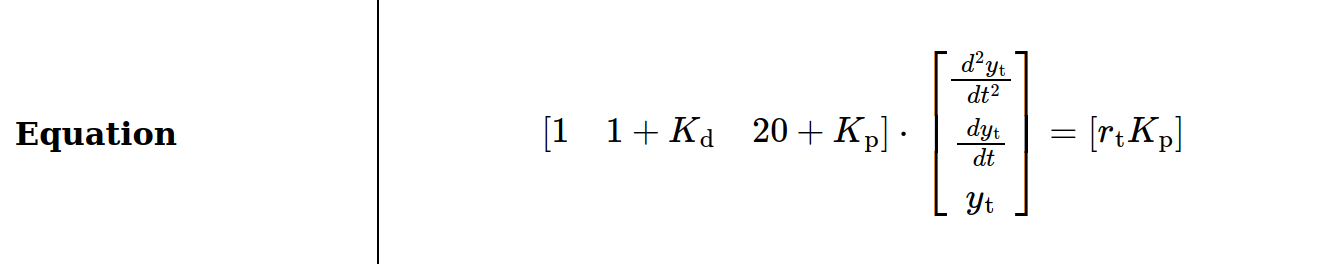
\includegraphics[width=1\textwidth]{figures/ODEInMatrix.png}
		\caption{Displaying ODE in a Matrix Form}
		\label{fig_multienv_odematrix}
	\end{subfigure}
	~
	\begin{subfigure}[t]{\textwidth}
		\centering
	
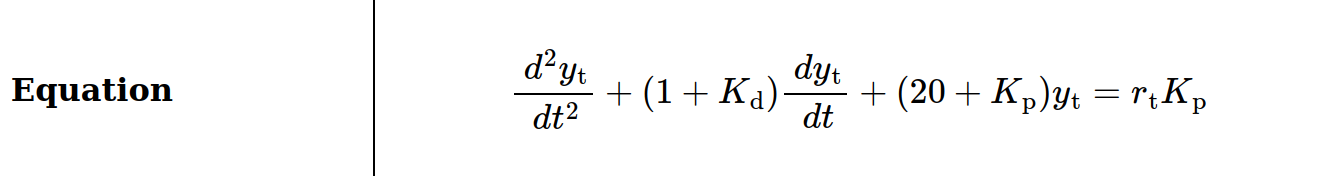
\includegraphics[width=1\textwidth]{figures/ODEInLinearEq.png}
		\caption{Displaying ODE as a Linear Equation}
		\label{fig_multienv_odelinear}
	\end{subfigure}
	
	\caption{Options of Displaying an ODE}
	\label{fig_multienv}
\end{figure}

1. We can display ODEs in a matrix form. The matrix form~\ref{eq_matrixformexmaple} is the prototype of how the ODE will appear in a matrix form in the SRS. In the \verb|DifferentialModel|, the \verb|_coefficients| is a list of lists \verb|Expr|, the unknown vector is a list of \verb|Unknown|, and the constant vector is a list of \verb|Expr|. It should be fairly straightforward for Drasil Printer to display them by printing each part sequentially. Figure~\ref{fig_multienv_odematrix} shows how to display a matrix of ODEs in the SRS. 

2. We also can display ODEs in a shape of a linear equation. Equation~\ref{eq_odeexmaple} is the prototype of how the ODE will show up in the shape of a linear equation in the SRS. Displaying a single ODE in a linear equation is a special case. When there is only one ODE, it would be over complicated to display it as a matrix. We explicitly force the Drasil printer to display a single ODE in the shape of a linear equation (Figure~\ref{fig_multienv_odelinear}). The example is just a demo that shows the Drasil printer is capable of displaying an ODE in a matrix form (Figure~\ref{fig_multienv_odematrix}).

In the future, the Drasil team wants to explore more variability in representing ODEs. An ODE has various forms, and we want \verb|DifferentialModel| to represent as many forms as possible. One topic highlighted in the discussion is showing an ODE in a canonical form. However, many mathematicians have different opinions on a canonical form, and the name of canonical form has been used differently, such as normal form or standard form. More research on this part would help us better understand the knowledge of ODE.
                  
    \setcounter{figure}{0}
    \setcounter{equation}{0}
    \setcounter{table}{0}

  \chapter{External libraries}
\label{cha_extlib}
External libraries are from an outside source; they do not originate from the source project. Our current interest is for libraries that are used to support solving scientific problems. We use external libraries to solve the ODE to save resources. Creating a complete ODE solver in Drasil would take considerable time, and there are already many reliable external libraries have been tested by long use. 

The external libraries are bodies of mathematical knowledge that are accessed through a well-defined interface. Since all external libraries are language-dependent, the Drasil framework needs to generate many interfaces to utilize external libraries. GOOL (Generic Object-Oriented Language) is the module to do this job. With the implementation of GOOL, the Drasil framework can generate five different languages: Python, Java, C\texttt{++}, C\#, and Swift. Among those five languages, four programming languages have ODE libraries for solving ODEs; we did not find a suitable library for Swift. In Python, the Scipy library~\citep{scipy} is a well-known scientific library for solving scientific problems, including support for solving ODEs. In Java, a library called Apache Commons Maths (ACM)~\citep{apache} provides a supplementary library for solving mathematical and statistical problems not available in the Java programming language. ACM includes support to solve ODEs. Two less known libraries to solve ODEs are the ODEINT Library~\citep{odeint} in C\texttt{++} and the OSLO Library~\citep{oslo} in C\#. There could be multiple external libraries to solve the ODE in one language, but we currently only support one library for each language.

We believe it is beneficial to conduct a commonalty analysis for all four selected libraries because the Drasil framework is suited to generate program families. A program families~\citep{dp1976} is a set of programs whose common properties are so extensive that it is advantageous to study the common properties of the programs before analyzing individual members. In this case, we may want to instruct the Drasil Code Generator to create programs that solve ODEs in multiple algorithms or allow other output types to interact with other modules. Those programs have parameterizable variabilities, so we can take advantage of developing them as a family~\citep{ss2004}.

The four selected libraries have commonalities and variabilities. Firstly, they all provide a numerical solution for a system of first-order ODEs. Each library can output a value of the dependent variable at a specific time, and we can collect those values in a time range. Secondly, they all provide different algorithms for solving ODEs numerically; we will conduct a rough commonality analysis of available algorithms in Section~\ref{se_algorithmoptiopns}. A complete commonality analysis would be too time-consuming and out of the scope of our study. Lastly, the OSLO library have the potential to output an ODE in different types. This discovery will provide options for the Drasil framework to solve an ODE by generating a library rather than a standalone executable program. 

This chapter will discuss topics related to the commonalities and variabilities of the four libraries, including numerical solutions, algorithms options and outputting an ODE in different types. 

\section{Numerical Solutions}
We use algorithms to make approximations for mathematical equations and create numerical solutions. All numerical solutions are approximations, and some numerical solutions that utilize better algorithms can produce better results than others. All selected libraries provide numerical solutions for a system of first-order ODEs as an IVP (Initial Value Problem). The IVP requires an initial condition that specifies the function's value at the start point, contrasting with a BVP (Boundary Value Problem). In a BVP, we apply boundary values instead of initial values. In this research, we will solve each scientific problem as an IVP. Let's see how to solve a system of first-order ODEs with an example. 

The following example is derived from Equation~\ref{eq_odeexmaple}. We transform the second-order ODE into a system of first-order ODEs. We replaced $y(t)$ with $x_{1}(t)$, and $y'(t)$ with $x_{2}(t)$. The details on how to convert a higher-order linear ODE to a system of first-order ODEs are shown in Section~\ref{se_hightofirst}. At this point, our goal is to show an example of how we encode a system of first-order ODEs in Drasil.

\begin{flalign} \label{ex_firstorderode}
& x_{1}'(t) = x_{2}(t) \\ \nonumber
& x_{2}'(t) = -(1 + K_{d}) \cdot x_{2}(t) - (20 + K_{p}) \cdot x_{1}(t) + r_{t} \cdot K_{p} 
\end{flalign}
\myequations{System of First-Order ODEs for PDContoller}

In Equation~\ref{ex_firstorderode}, there are two dependent variables: $x_1$ and $x_2$. Both $x_1(t)$ and $x_2(t)$ are functions of the independent variable, in this case time $t$. $x_1$ is the process variable, and $x_2$ is the rate of change of $x_1$. $x_1'$(t) is the first directive of the function $x_1(t)$ with respect to time, and $x_2'$(t) is the first derivative of the function $x_2$(t) with respect to time. $K_d$, $K_p$, and $r_t$ are constant variables; they have the same meaning as in Equation~\ref{eq_odeexmaple} and Equation~\ref{ex_firstorderode}. We can encode Equation~\ref{ex_firstorderode} in all four libraries.

In Python Scipy library, we can write the example as follows:
\begin{python1}
def f(t, y_t):
    return [y_t[1], -(1.0 + K_d) * y_t[1] + -(20.0 + K_p) * y_t[0] + r_t * K_p]
\end{python1}
In this example, $y\_t$ is a list of dependent variables. The index 0 of $y\_t$ is the dependent variable $x_1$, and the index 1 of $y\_t$ is the dependent variable $x_2$. $y\_t[1]$ represent the first equation $x_{1}'(t) = x_{2}(t)$ in Equation~\ref{ex_firstorderode}. The second value in the returned list $(-(1.0 + K\_d) * y\_t[1] + -(20.0 + K\_p) * y\_t[0] + r\_t * K\_p)$ represents the second equation, $x_{2}'(t) = -(1 + K_{d}) \cdot x_{2}(t) - (20 + K_{p}) \cdot x_{1}(t) + r_{t} \cdot K_{p}$, in Equation~\ref{ex_firstorderode}. 

In Java ACM library, we can write the example using the following code:
\begin{java1}
public void computeDeriv(double t, double[] y_t, double[] dy_t) {
    dy_t[0] = y_t[1];
    dy_t[1] = -(1.0 + K_d) * y_t[1] + -(20.0 + K_p) * y_t[0] + r_t * K_p;
}
\end{java1}

In C\texttt{++} ODEINT library, we can write the example as the following code:
\begin{cplusplus1}
void ODE::operator()(vector<double> y_t, vector<double> &dy_t, double t) {
    dy_t.at(0) = y_t.at(1);
    dy_t.at(1) = -(1.0 + K_d) * y_t.at(1) + -(20.0 + K_p) * y_t.at(0) + r_t * K_p;
}	
\end{cplusplus1}

In C\# OSLO library, we can write the example as the following code:
\begin{csharp1}
Func<double, Vector, Vector> f = (t, y_t_vec) => {
    return new Vector(y_t_vec[1], -(1.0 + K_d) * y_t_vec[1] + -(20.0 + K_p) * y_t_vec[0] + r_t * K_p);
};
\end{csharp1}

Once we capture the information of the system of ODEs, we have to give an initial condition for solving an ODE as an IVP. To solve Equation~\ref{ex_firstorderode}, we must provide the initial value for both $x_1$ and $x_2$. Overall, an ODE is a simulation, and it simulates a function of time. Before we start the simulation, other configurations need to be specified, including the start time, end time, and time step between each iteration. We can also provide values for each library's absolute and relative tolerance. Those two tolerances control the accuracy of the solution. As we mentioned before, all numerical solutions are approximations. High tolerances produce less accurate solutions, and smaller tolerances produce more accurate solutions. Lastly, we have to collect the numerical output for each iteration. The full details on how each library solves Equation~\ref{ex_firstorderode} are shown in Appendix~\ref{numsol} and Code~\ref{code_csharposlo}.

\section{Algorithm Options}
\label{se_algorithmoptiopns}
We can solve an ODE with many algorithms. The four selected libraries each provide many algorithms. We roughly classify available algorithms into four categories based on the type of algorithm they use. They are a family of Adams methods, a family of backward differentiation formula methods (BDF), a family of Runge-Kutta (RK) methods, and a ``catch all'' category of other methods. The commonality analysis we provide on available algorithms is a starting point. It is an incomplete approximation. Getting a complete commonality analysis will require help from domain experts in ODE. Although the commonality is incomplete, the team still benefits from the current analysis. Not only can a future student quickly access information on which algorithm is available in each language, but also the analysis reminds us that we can increase the consistency of artifacts by providing one-to-one mapping for each algorithm in the four libraries. For example, if a user explicitly chooses a family of Adams methods as the targeted algorithm, all available libraries should use a family of Adams methods to solve the ODE. Unfortunately, not all libraries provide a family of Adams methods. The targeted algorithm will affect what languages we can generate. Table~\ref{tab_algoexlib} shows the availability of a family of algorithms in each library. The full details of each library's algorithm availability are shown in Appendix~\ref{alg_externallib}.

\begin{sidewaystable}
\begin{adjustbox}{width=\columnwidth,center}
\begin{tabular}{p{0.18\textwidth} | p{0.22\textwidth} p{0.22\textwidth} p{0.29\textwidth} p{0.25\textwidth}}\hline
    \backslashbox{Algorithm}{Library}
    &\textbf{Scipy-Python}&\textbf{ACM-Java}&\textbf{ODEINT-C\texttt{++}}&\textbf{OSLO-C\#}\\
    \toprule
    Family of Adams & 
        \begin{itemize}[wide]
        \item Implicit Adams
        \end{itemize} & 
        \begin{itemize}[wide]
        \item Adams Bashforth
        \item Adams Moulton
        \end{itemize} & 
        \begin{itemize}[wide]
        \item Adams Bashforth Moulton
        \end{itemize} &\\ \hline
    Family of BDF & 
        \begin{itemize}[wide]
        \item BDF
        \end{itemize} &&& 
        \begin{itemize}[wide]
        \item Gear’s BDF
        \end{itemize} \\ \hline
    Family of RK & 
        \begin{itemize}[wide]
        \item Dormand Prince (4)5 
        \item Dormand Prince 8(5,3) 
        \end{itemize} & 
        \begin{itemize}[wide]
        \item Explicit Euler
        \item 2ed order
        \item 4th order
        \item Gill fourth order
        \item 3/8 fourth order
        \item Luther sixth order
        \item Higham and Hall 5(4)
        \item Dormand Prince 5(4) 
        \item Dormand Prince 8(5,3) 
        \end{itemize} & 
        \begin{itemize}[wide]
        \item Explicit Euler
        \item Implicit Euler
        \item Symplectic Euler
        \item 4th order
        \item Dormand Prince 5
        \item Fehlberg 78
        \item Controlled Error Stepper
        \item Dense Output Stepper
        \item Rosenbrock 4
        \item Symplectic RKN McLachlan 6
        \end{itemize} & 
        \begin{itemize}[wide]
        \item Dormand Prince RK547M
        \end{itemize} \\ \hline
    Others && 
        \begin{itemize}[wide]
        \item Gragg Bulirsch Stoer 
        \end{itemize} & 
        \begin{itemize}[wide]
        \item Gragg Bulirsch Stoer 
        \end{itemize} &\\
    \bottomrule	
\end{tabular}
\end{adjustbox}
\caption{Algorithms Support in External Libraries}	
\label{tab_algoexlib}
\end{sidewaystable}

\section{Output an ODE}
In the Drasil framework, there is an option to generate modularized software. This modularized software currently contains a controller module, an input module, a calculation module, and an output module. The controller module contains the main function that starts the software. The input module handles all input parameters and constraints. We manually create a text file that contains all input information. For example, in Double Pendulum, the input module will read Code~\ref{code_inputfile} and convert the information to its environment. 

\begin{listing}[ht]
\begin{python1}
# Length of the upper rod (m)
2.0
# Length of the bottom rod (m)
1.0
# Mass of the upper object(kg)
0.5
# Mass of the bottom object(kg)
2.0
\end{python1}
\captionof{listing}{A Sample Input File for Double Pendulum}
\label{code_inputfile}
\end{listing}

The calculation module contains all the logic for solving the scientific problem. For example, in Double Pendulum, the calculation module contains all functions for calculating the numerical solution. Lastly, the output module will output the solution. In all ODE case studies, the output module will write the values returned by the calculation module as a string. For example, in Double Pendulum, the output module write Code~\ref{code_outputfile} in a text file.

\begin{listing}[ht]
\begin{python1}
# this is theta 1
theta = [1.3463968515384828, 1.3463947169563892, 1.346388313227267, 1.3463776404025904, 1.3463626985681507, 1.3463434878440559, ... ]
\end{python1}
\captionof{listing}{A Output File for Double Pendulum}
\label{code_outputfile}
\end{listing}

With each module interacting with others we would like to study the output of the calculation module in the ODE case studies. Currently, the calculation module will output a finite sequence of real numbers, $\mathbb{R}^m$, for example, a list of numbers in Python. $m$ is a natural number which depends on the start time, end time, and time step. We have the following specification for the calculation module:

\begin{table}[ht]
\centering
\begin{tabular}{p{0.2\textwidth} | p{0.3\textwidth} | p{0.3\textwidth}} \hline
    \textbf{Module Name}&\textbf{Input}&\textbf{Output}\\
    \toprule
    Calculations & $\mathbb{R}^n$ & $\mathbb{R}^m$ \\
    \bottomrule	
\end{tabular}	
\caption{Specification for Calculations Module Returns a Finite Sequence}	
\label{tab_srsforcal}
\end{table}
$\mathbb{R}^n$ represents input values, and the superscript $n$ means how many input values. In our case study, after running the generated program, it will create a file containing the numerical solution of the ODE from the start time to the end time. The numerical solution is written as a stream of real numbers in Code~\ref{code_outputfile}. A finite sequence of real numbers only captures a partial solution; we ideally want to capture a complete solution. Therefore, we would like to explore options to output a different type for the calculation module.

Most selected external libraries only provide numerical solutions in the form of a finite sequence of real numbers, $\mathbb{R}^m$. The C\# OSLO library not only supports outputting a finite sequence of real numbers but also an infinite sequence of real numbers (we use \verb|double| as the type for real numbers in C\# code). In C\# OSLO library, we can get an infinite numerical solution that contains all possible values of the dependent variable over time ($\mathbb{R}^{\infty}$). $\infty$ is the length of the sequence, and it is a natural number. The function \verb|Ode.RK547M| returns an endless enumerable sequence of solution points. If we are interested in a partial solution ($\mathbb{R}^m$), we can filter it with parameters such as start time, end time, and time step. Code~\ref{code_csharposlo} shows the full details of how to solve Equation~\ref{ex_firstorderode} in the OSLO library.
\begin{listing}[ht]
\begin{csharp1}
public static List<double> func_y_t(double K_d, double K_p, double r_t, double t_sim, double t_step) {
    List<double> y_t;
    Func<double, Vector, Vector> f = (t, y_t_vec) => {
        return new Vector(y_t_vec[1], -(1.0 + K_d) * y_t_vec[1] + -(20.0 + K_p) * y_t_vec[0] + r_t * K_p);
    };
    Options opts = new Options();
    opts.AbsoluteTolerance = Constants.AbsTol;
    opts.RelativeTolerance = Constants.RelTol;
    
    Vector initv = new Vector(new double[] {0.0, 0.0});
    IEnumerable<SolPoint> sol = Ode.RK547M(0.0, initv, f, opts);
    IEnumerable<SolPoint> points = sol.SolveFromToStep(0.0, t_sim, t_step);
    y_t = new List<double> {};
    foreach (SolPoint sp in points) {
        y_t.Add(sp.X[0]);
    }
    
    return y_t;
}
\end{csharp1}
\captionof{listing}{Source Code of Solving PDController in OSLO}
\label{code_csharposlo}
\end{listing}

In Code~\ref{code_csharposlo}, between line 3 and line 4, we encode the ODE of Equation~\ref{ex_firstorderode} in a \verb|Func|. Between line 7 and line 8, we set the absolute and relative tolerance in the \verb|Options| class. In line 10, we initialize initial values. Next, in line 11, we use \verb|Ode.RK547M| to get an endless sequence of real numbers, $\mathbb{R}^{\infty}$. In line 12, we use \verb|SolveFromToStep| to get a partial solution ($\mathbb{R}^m$) based on the start time, the final time, and the time step. Last, between line 13 and line 15, we run a loop to collect the process variable $x_1$. With the workflow we described above, the \verb|Ode.RK547M(0.0, initv, f, opts)| returns an object with richer data because {}$\mathbb{R}^m \subset \mathbb{R}^{\infty}$. Instead of returning $\mathbb{R}^m$, we can have an option to return $\mathbb{R}^{\infty}$. Here is the new specification.

\begin{table}[ht]
\centering
\begin{tabular}{p{0.2\textwidth} | p{0.3\textwidth} | p{0.3\textwidth}} \hline
    \textbf{Module Name}&\textbf{Input}&\textbf{Output}\\
    \toprule
    Calculations & $\mathbb{R}^n$ & $\mathbb{R}^{\infty}$ \\
    \bottomrule	
\end{tabular}	
\caption{Specification for Calculations Module Return an Infinite Sequence}	
\label{tab_srsforcal}
\end{table}
The implementation of this specification is not complete, but we provide an analysis of what options the C\# OSLO library offers.

Ideally, the ODE is a function that means giving an independent variable will output dependent variables. Here is another proposed specification:
\begin{table}[ht]
\centering
\begin{tabular}{p{0.2\textwidth} | p{0.3\textwidth} | p{0.3\textwidth}} \hline
    \textbf{Module Name}&\textbf{Input}&\textbf{Output}\\
    \toprule
    Calculations & $\mathbb{R}^n$ & $\mathbb{R} \rightarrow \mathbb{R}^k$ \\
    \bottomrule	
\end{tabular}	
\caption{Specification for Calculations Return a Funtion}	
\label{tab_srsforcal}
\end{table}

In output $\mathbb{R} \rightarrow \mathbb{R}^k$, $\mathbb{R}$ is the independent variable, and $\mathbb{R}^k$ is a sequence that contains dependent variables. For a fourth-order ODE, $\mathbb{R}^k$ would be $\mathbb{R}^4$. Since Drasil Framework can generate a library, the idea of outputting an ODE as a function can be useful. A program can hook up the interface of the generated library, and the library will provide support for calculating the numerical solution of the ODE. The implementation of this specification is not complete, but it gives future students some inspiration on how to generate a library to solve the ODE in Drasil. We defined how to generate the code for external libraries in Drasil Code Generator. To generate new interfaces for each library in each language, future students need to write new instructions. 
                  
    \setcounter{figure}{0}
    \setcounter{equation}{0}
    \setcounter{table}{0}

  \chapter{Connect Model to Libraries}
We store the information of a higher-order linear ODE in the \verb|DifferentialModel| in Chapter 2. This \verb|data type| captures the structure of the ODE so that we can transform the ODE into other forms. Chapter 3 discusses how to solve a system of first-order ODEs numerically in four selected external libraries. However, there is a gap between the \verb|DifferentialModel| and external libraries. The selected libraries cannot solve the higher-order ODE directly, but they can solve its equivalent system of first-order equations. We know that most ways of solving ODEs are intended for systems of first-order ODEs, so we want to convert the higher-order ODE to a system of first-order ODEs~\citep{converthigherode}. Firstly, we transform a linear higher-order ODE into a system of first-order ODEs. Then, we use the Drasil Code Generator to generate code that contains proper interfaces for utilizing four selected external libraries. This program solves the system of first-order ODEs numerically by producing a list of values of dependent variables based on time. The original linear higher-order ODE is equivalent to the system of first-order linear ODEs we solve. Thus, by transitivity, the numerical solution for the system of first-order ODEs is also the numerical solution of the higher-order ODE.

In this research, my work primarily focuses on enabling the Drasil Code Generator to generate code for solving higher order ODE and automatically extracting useful information from \verb|DifferentialModel| for the Drasil Code Generator in single higher-order linear ODEs. In addition, we create a new case study, Double Pendulum, which has a system of nonlinear ODEs. We handle the nonlinear ODE differently than the linear ODE. The nonlinear ODE still requires Drasil users manually extract information from the original ODE. With the new implementations, we can generate code to solve the Double Pendulum numerically. In this chapter, we will first discuss how to convert any higher-order linear ODE to a system of first-order ODEs in theory. Then, we will discuss how to enable the Drasil Code Generator to generate code that produces a numerical solution for a system of first-order ODEs. Lastly, we will discuss how to automate the generation process.

\section{Higher Order to First Order}
\label{se_hightofirst}
Any higher-order linear ODE can be written in the following form:
\begin{equation} \label{eq_isohighode}
  y^n = f (t, y, y', y'', \dots, y^{\textit{(n-1)}})
\end{equation}

We isolate the highest derivative $y^n$ on the left-hand side and move the rest of the terms to the right-hand side. On the right-hand side, $f (t, y, y', y'', \dots, y^{\textit{(n-1)}})$ means a function depends on variables $t$, $y$, $y'$, $\dots$, and $y^{\textit{(n-1)}}$. $t$ is the independent variable, often time. $y$, $y'$, $\dots$, and $y^{\textit{(n-1)}}$ represent the dependent variable $y$, the first derivative of $y$, $\dots$, up to $(n-1)^\text{th}$ derivative.

For the next step, we introduce the following new variables: $x_{1}$, $x_{2}$, $\dots$, $x_{n}$. The number of newly introduced dependent variables equals the order of the ODE, $n$. The new relationship is shown below:
\begin{flalign} \label{eq_newvars}
  & x_{1} = y \\ \nonumber
  & x_{2} = y' \\ \nonumber
  & \dots \\ \nonumber
  & x_{n} = y^{\textit{(n-1)}} 
\end{flalign}

Next, we differentiate $x_{1}$, $x_{2}$, $\dots$, $x_{n}$ in Equation~\ref{eq_newvars} to establish the following relationships between the variables:
\begin{flalign} \label{eq_diffvervars}
  & x_{1}' = y' = x_{2} \\ \nonumber
  & x_{2}' = y'' = x_{3} \\ \nonumber
  & \dots \\ \nonumber
  & x_{n-1}' = y^{\textit{(n-1)}} = x_{n}\\ \nonumber
  & x_{n}' = y^{n} = f (t, x_{1}, x_{2}, \dots, x_{n})
\end{flalign}

Since the higher-order ODE is a linear ODE, $f (t, x_{1}, x_{2}, \dots, x_{n})$ is a linear function; therefore, we can rewrite $f (t, x_{1}, x_{2}, \dots, x_{n})$ as
\begin{equation}\label{eq_linear}
b_{0}(t) \cdot x_{1} + b_{1}(t) \cdot x_{2} + \dots + b_{n-1}(t) \cdot x_{n} + h(t)
\end{equation}
where $b_{0}(t)$, $\dots$, $b_{n-1}(t)$ and $h(t)$ are constant functions or non-constant functions.

Based on Equation~\ref{eq_diffvervars} and Equation~\ref{eq_linear}, we obtain:
\begin{flalign} \label{eq_diffvervarslinear}
    & x_{1}' = x_{2} \\ \nonumber
    & x_{2}' = x_{3} \\ \nonumber
    & \dots \\ \nonumber
    & x_{n-1}' = x_{n}\\ \nonumber
    & x_{n}'= b_{0}(t) \cdot x_{1} + b_{1}(t) \cdot x_{2} + ... + b_{n-1}(t) \cdot x_{n} + h(t)
\end{flalign}

We can rewrite Equation~\ref{eq_diffvervarslinear} in a general form:
\begin{equation} \label{eq_foode}
  \boldsymbol{x}' = \boldsymbol{Ax} + \boldsymbol{c}
\end{equation}
\myequations{System of First-Order ODEs in a General Form}
The $\boldsymbol{A}$ is a coefficient matrix, and $\boldsymbol{c}$ is a constant vector. The $\boldsymbol{x}$ is the unknown vector that contains functions of the independent variable, often time. The $\boldsymbol{x'}$ is a vector that consists of the first derivatives of $\boldsymbol{x}$. The following is the long matrix form:
\begin{equation} \label{eq_foodeexample}
	\begin{bmatrix}
		x_{1}' \\
    x_{2}' \\
    \dots  \\
    x_{n-1}' \\
    x_{n}'
	\end{bmatrix}
    = 
  \begin{bmatrix}
		0, & 1, & 0, & \dots & 0 \\
    0, & 0, & 1, & \dots & 0 \\
    \dots \\
    0, & 0, & 0, & \dots & 1 \\
    b_{0}(t), & b_{1}(t), & b_{2}(t), & \dots & b_{n-1}(t)
	\end{bmatrix}
    \cdot
  \begin{bmatrix}
		x_{1} \\
    x_{2} \\
    \dots  \\
    x_{n-1} \\
    x_{n}
	\end{bmatrix}
    + 
  \begin{bmatrix}
    0 \\
    0 \\
    \dots  \\
    0 \\
    h(t)
	\end{bmatrix}
\end{equation}

\section{Connect Drasil with External Libraries}
\label{se_connecteetolib}

In previous research, Drasil developers wrote the ODE as a \href{https://jacquescarette.github.io/Drasil/docs/full/drasil-lang-0.1.60.0/Language-Drasil-Chunk-Relation.html#t:RelationConcept}{RelationConcept} \verb|data type|, which has a field called \verb|_rel|. The \verb|_rel| is \href{https://jacquescarette.github.io/Drasil/docs/full/drasil-lang-0.1.60.0/Language-Drasil-ModelExpr-Lang.html#t:ModelExpr}{ModelExpr} type and can be used for representing mathematical expressions. We can write mathematical expressions such as the right-hand side equal to the left-hand side in \verb|ModelExpr|. The drawback is that we cannot extract useful information from \verb|RelationConcept| to allow the Drasil Code Generator to utilize that information. The Drasil printer can print a \verb|RelationConcept| in the SRS, but the Drasil Code Generator cannot utilize the \verb|RelationConcept|. Therefore, in the previous approach, the user has to repeat information through a manually created \verb|data type|, called \href{https://jacquescarette.github.io/Drasil/docs/drasil-code-0.1.9.0/Language-Drasil-Code.html#t:ODEInfo}{ODEInfo}, to generate code. Our improved approach expanded the Drasil Code Generator's capability to generate code for solving a higher-order ODE.

\subsection{Enable Drasil for Solving Higher-Order ODEs}
The Drasil Code Generator utilized \verb|ODEInfo| to generate code which produces a numerical solution. We can find details on how to generate code that solves a first-order ODE numerically in Brooks's thesis (91-103)~\citep{brooks}. His work could generate code for a first-order ODE but not a higher-order ODE. A McMaster student, Naveen, created the \href{https://jacquescarette.github.io/Drasil/examples/pdcontroller/SRS/srs/PDController_SRS.html}{PDContoller}. It generates code for solving a second-order linear ODE numerically in Python only. The new approach will generate code for solving any higher-order linear ODE in Python, Java, C\texttt{++} and C\#.

Before our changes, \verb|ODEInfo| only had an option to provide one initial value. For a higher-order ODE, the current setting of \verb|ODEInfo| does not hold all information we need. \verb|ODEInfo| needs to store multiple initial values to enable the Drasil Code Generator to work for the higher-order ODE. For example, we need four initial values when we solve a fourth-order ODE as an IVP. Thus, the Drasil Code Generator must adapt to handle multiple initial values.

\begin{listing}[ht]
\begin{haskell1}
-- Old 
data ODEInfo = ODEInfo {
  ...
  initVal :: CodeExpr
  ...
}

-- New 
data ODEInfo = ODEInfo {
  ...
  initVal :: [CodeExpr],
  ...
}
\end{haskell1}
\captionof{listing}{Source Code for Initial Values in Drasil}
\label{code_odeinfointial}
\end{listing}
Code~\ref{code_odeinfointial} changes the \verb|data type| of \verb|initVal| from a \verb|CodeExpr| to a list of \verb|CodeExpr|. Users can only set one initial value in the old way, but now they can set a list of multiple initial values. This change allows Drasil users to store multiple initial values in a list. We also have to ensure that Drasil Code Generator can utilize the new \verb|data type| \verb|[CodeExpr]|. Previously, Drasil Code Generator only handled the \verb|initVal| as \verb|CodeExpr|. Now the \verb|initVal| becomes \verb|[CodeExpr]|. In the Drasil framework, we handle a list of \verb|data type| by \href{https://jacquescarette.github.io/Drasil/docs/drasil-code-base-0.1.9.0/Language-Drasil-CodeExpr.html#v:matrix}{matrix} (In Drasil the \verb|data type| \verb|matrix| is used to represent both a 1D matrix (conventionally called a vector) and a 2D matrix.), and the code \verb|initVal info| retrieves the \verb|initVal| from the \verb|ODEInfo| \verb|data type|. The \verb|matrix| can wrap a \verb|[CodeExpr]| into a \verb|CodeExpr|. 

\begin{listing}[ht]
\begin{haskell1}
matrix[initVal info]
\end{haskell1}
\end{listing}

In \verb|initSolListWithValFill|, \verb|basicArgFill|, and \verb|CodeDefinition| for \verb|ODEInfo|, we have to ensure we wrap the \verb|initVal|.
% We need to change multiple functions to ensure the Drasil Code Generator adapts a list of values. 

% We need to change \verb|initSolListWithValFill|(97)~\citep{brooks}, \verb|basicArgFill|(96,98)~\citep{brooks}

% The first function is \verb|initSolListWithValFill|(97)~\citep{brooks}. Since we change the type of \verb|initVal| to a list of \verb|CodeExpr|, we need to use \verb|matrix| to wrap \verb|[initVal info]| as a \verb|CodeExpr|. We use \verb|initSolListWithValFill| for generating interfaces in the Scipy Library.
% \begin{listing}[ht]
% \begin{haskell1}
% -- Old 
% initSolListWithValFill (depVar info) (initVal info)

% -- New 
% initSolListWithValFill (depVar info) (matrix[initVal info]) 
% \end{haskell1}
% \end{listing}

% The second function is \verb|basicArgFill|(96,98)~\citep{brooks}, which takes a CodeExpr. We use \verb|basicArgFill| for filling values for variables and \verb|matrix| to wrap \verb|[initVal info]| as a \verb|CodeExpr|.

% \begin{listing}[ht]
% \begin{haskell1}
% basicArgFill :: CodeExpr -> ArgumentFill
% basicArgFill = BasicF
% \end{haskell1}
% \end{listing}

% \begin{listing}[ht]
% \begin{haskell1}
% -- Old 1
% basicArgFill[initVal info] -- page 96

% -- Old 2
% basicArgFill [matrix[[initVal info]] -- page 98

% -- New 
% basicArgFill matrix [initVal info]
% \end{haskell1}
% \end{listing}
The change of \verb|basicArgFill| impacts generated code in the Python Scipy library and C\# OSLO library. For the Python Scipy library, in Code~\ref{code_pythonintial}, line 6 sets the initial value with a list of \verb|T_init|.

\begin{listing}
\begin{python1}
# Old 
  r.set_initial_value(T_init, 0.0)
  T_W = [T_init]

# New 
  r.set_initial_value([T_init], 0.0)
  T_W = [[T_init][0]] # Initial values are also a part of the numerical solution, so we have to add the proper initial value to the list.
\end{python1}
\captionof{listing}{Source Code for Initial Values in Python}
\label{code_pythonintial}
\end{listing}
The same thing happens in C\# OSLO. In Code~\ref{code_csharpintial}, line 5 initializes a list \verb|T_init|, and we later use it as the initial values.  
\begin{listing}[ht]
\begin{csharp1}
// Old 
Vector initv = new Vector(T_init);

// New 
Vector initv = new Vector(new double[] {T_init});
\end{csharp1}
\captionof{listing}{Source Code for Initial Values in C\#}
\label{code_csharpintial}
\end{listing}

In the Java ACM library, we use the \href{https://commons.apache.org/proper/commons-math/apidocs/org/apache/commons/math4/ode/FirstOrderDifferentialEquations.html}{FirstOrderDifferentialEquations} interface to solve a system of first-order ODEs. This interface has a method called \verb|getDimension()|. In the previous implementation, the \verb|getDimension()| will always return 1 because we only solve a first-order ODE. It has been hard-coded in the Drasil Code Generator. Since we want to solve a $n^{th}$-order ODE, the \verb|getDimension()| needs to return $n$.

\begin{listing}
\begin{java1}
// Old 
public class ODE implements FirstOrderDifferentialEquations {
  ...
  public int getDimension() {
    return 1;
  }
}
// New 
public class ODE implements FirstOrderDifferentialEquations {
  ...
  public int getDimension() {
    return n; // n is an integer that users can explicitly define
  }
}
\end{java1}
\captionof{listing}{Source Code for Returning Dimension in Java}
\label{code_javadimen}
\end{listing}

To allow \verb|getDimension()| to return an integer based on the order of the ODE, we have to add two additional methods based on function \verb|fixedReturn|(100)~\citep{brooks} and fixedStatementFill(89)~\citep{brooks} in the Drasil Code Generator. The \verb|fixedReturn| indicates a step that returns a fixed value, such as \verb|fixedReturn (int 1)|. We create similar methods \verb|fixedReturn'| and \verb|fixedStatementFill'|. In Code~\ref{code_fixedreturn}, the \verb|fixedReturn'| will indicate a step that returns a fixed value, but the \verb|fixedStatementFill'| will fill in the fixed value base on the order of the ODE. Now, in Code~\ref{code_javadimen}, line 12, $n$ will depends on the value we pass in \verb|fixedStatementFill'|.

\begin{listing}
\begin{haskell1}
-- Old 
fixedReturn :: CodeExpr -> Step
fixedReturn = lockedStatement . FRet

fixedStatementFill :: StepFill
fixedStatementFill = StatementF [] []

-- New added 
fixedReturn' = statementStep (\cdchs [e] -> case (cdchs, e) of
  ([], _) -> FRet e
  (_,_) -> error "Fill for fixedReturn' should provide no CodeChunk")

fixedStatementFill' :: CodeExpr -> StepFill
fixedStatementFill' a = StatementF [] [a]
\end{haskell1}
\captionof{listing}{Source Code for Returning a Fixed Value}
\label{code_fixedreturn}
\end{listing}

In C\texttt{++}, the backend code already handles the initial value as a list, so there is no change for artifacts.

% Lastly, we have to redefine \verb|CodeDefinition| for \verb|ODEInfo|(118)~\citep{brooks}. We use \verb|CodeDefinition| in the Drasil Generator to map variables between \verb|ODEInfo| and generated code. In Code~\ref{code_odeinfocodedef}, we used \verb|matrix| to wrap \verb|[initVal info]| as a \verb|CodeExpr|.

% \begin{listing}
% \begin{haskell1}
% -- Old 
% odeDef :: ODEInfo -> CodeDefinition
% odeDef info = CD 
%   ...
%   (map ($ info) [tInit, tFinal, initVal, absTol . odeOpts, 
%   relTol . odeOpts, stepSize . odeOpts]) 
%   ODE

% -- New 
% odeDef :: ODEInfo -> CodeDefinition
% odeDef info = CD 
%   ...
%   (matrix [initVal info]: map ($ info) [tInit, tFinal, absTol . odeOpts, relTol . odeOpts, stepSize . odeOpts])
%   ODE
% \end{haskell1}
% \captionof{listing}{Source Code for ODEInfo CodeDefinition}
% \label{code_odeinfocodedef}
% \end{listing}

Allowing multiple initial values unlocks the potential for Drasil to generate code that produces the numerical solution for a system of first-order ODEs. Every higher-order linear ODE has its equivalent system of first-order ODEs, and the solution for the system of first-order ODEs is also the solution for the higher-order ODE. The same thing happens on nonlinear higher-order ODEs. If we can transform a higher-order nonlinear ODE into a system of first-order ODEs, we can solve it via the four selected external libraries. For nonlinear ODEs, the process is not so automated; the user will need to do some manual work, as explained through the Double Pendulum example.

\subsection{Double Pendulum}
\label{se_dblpen}
Figure~\ref{fig_dblpen} demonstrates how a double pendulum works in a lab environment. The full details of the Double Pendulum's SRS are located on the \href{https://jacquescarette.github.io/Drasil/examples/dblpendulum/SRS/srs/DblPendulum_SRS.html}{Drasil website}. Table~\ref{tab_dblpendes} lists all variables in the Double Pendulum example.
\begin{figure}[ht]
  \centering
  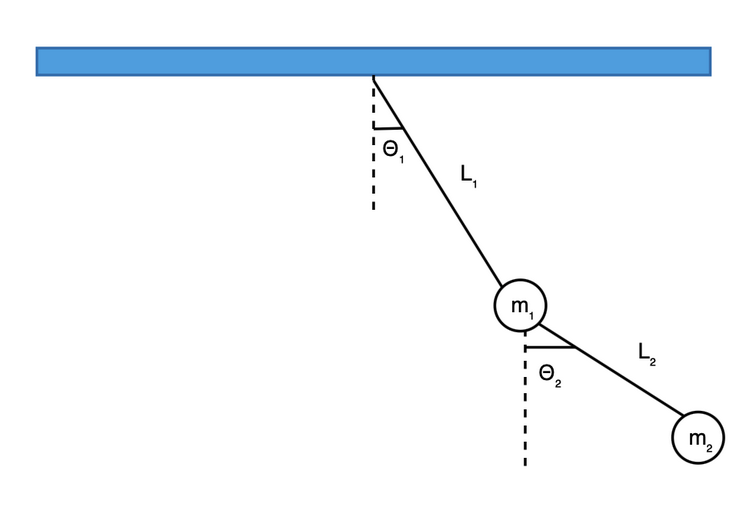
\includegraphics[width=0.6\textwidth]{figures/DblPendulum.png}
  \caption{Double Pendulum Demonstration}
  \label{fig_dblpen}
\end{figure}

\begin{table}[ht]
	\begin{tabular}{ p{0.2\textwidth} p{0.7\textwidth} }
		\textbf{Name} & \textbf{Description} \\
		\toprule
		\verb|m₁| & The mass of the first object\\
    \verb|m₂| & The mass of the second object\\
		\verb|L₁| & The length of the first rod\\
		\verb|L₂| & The length of the second rod\\
		\verb|g| & Gravitational acceleration\\
		\verb|θ₁| & The angle of the first rod\\
		\verb|θ₂| & The angle of the second rod\\
		\verb|ω₁| & The angular velocity of the first object\\
		\verb|ω₂| & The angular velocity of the second object\\
		\bottomrule	
	\end{tabular}	
	\caption{Variables in Double Pendulum Example}	
	\label{tab_dblpendes}
\end{table}

At this point, we have primarily focused on solving linear ODEs. Despite the \href{https://jacquescarette.github.io/Drasil/examples/dblpendulum/SRS/srs/DblPendulum_SRS.html#Sec:IMs}{Double Pendulum case study} contains a nonlinear ODE, the Drasil framework can still generate code to solve it numerically with some additional help from the user. 

In the Double Pendulum case study, we want to solve the following equations:
\begin{flalign} \label{eq_dblpenhigh}
  & \theta_{1}'' = \frac{-g(2m_{1}+m_{2})\sin \theta_{1}-m_{2}g\sin (\theta_{1}-2\theta_{2})-2\sin (\theta_{1}-\theta_{2})m_{2}({\theta_{2}'}^2L_{2}+{\theta_{1}'}^2L_{1}\cos (\theta_{1}-\theta_{2}))}{L_{1}(2m_{1}+m_{2}-m_{2}\cos (2\theta_{1}-2\theta_{2}))} \\ \nonumber
  & \theta_{2}'' = \frac{2\sin (\theta_{1}-\theta_{2})({\theta_{1}'}^2L_{1}(m_{1}+m_{2})+g(m_{1}+m_{2})\cos \theta_{1} + {\theta_{2}'}^2L_{2}m_{2}\cos (\theta_{1}-\theta_{2}))}{L_{2}(2m_{1}+m_{2}-m_{2}\cos (2\theta_{1}-2\theta_{2}))}
\end{flalign}
\myequations{Double Pendulum Equation}
There are two second-order ODEs in one system. To solve this system of ODEs, we convert them into a system of first-order ODEs. The transformation follows the methodology we discussed in Section~\ref{se_hightofirst}. We transform Equation~\ref{eq_dblpenhigh} into Equation~\ref{eq_dblpenfirst}. Once the transformation is complete, we can encode Equation~\ref{eq_dblpenfirst} and pass it to the Drasil Code Generator. However, we cannot show Equation~\ref{eq_dblpenfirst} in the shape of Equation~\ref{eq_foode} because the ODE is not a linear ODE.

\begin{flalign} \label{eq_dblpenfirst}
  & \theta_{1}' = \omega_{1} \\ \nonumber
  & \theta_{2}' = \omega_{2} \\ \nonumber
  & \omega_{1}' = \frac{-g(2m_{1}+m_{2})\sin \theta_{1}-m_{2}g\sin (\theta_{1}-2\theta_{2})-2\sin (\theta_{1}-\theta_{2})m_{2}({\omega{2}}^2L_{2}+{\omega{1}}^2L_{1}\cos (\theta_{1}-\theta_{2}))}{L_{1}(2m_{1}+m_{2}-m_{2}\cos (2\theta_{1}-2\theta_{2}))} \\ \nonumber
  & \omega_{2}' = \frac{2\sin (\theta_{1}-\theta_{2})({\omega_{1}}^2L_{1}(m_{1}+m_{2})+g(m_{1}+m_{2})\cos \theta_{1} + {\omega_{2}}^2L_{2}m_{2}\cos (\theta_{1}-\theta_{2}))}{L_{2}(2m_{1}+m_{2}-m_{2}\cos (2\theta_{1}-2\theta_{2}))}
\end{flalign}
\myequations{Double Pendulum Equation in a System of First-Order ODEs}

Now that we have obtained Equation~\ref{eq_dblpenfirst}, we can encode it in Drasil. Code~\ref{code_encodedblpend} shows the example of how we encode Equation~\ref{eq_dblpenfirst} in Drasil. We replace the Drasil language with mathematical symbols to increase the readability of the code.
\begin{listing}[ht]
\begin{haskell1}
dblPenODEInfo :: ODEInfo
dblPenODEInfo = odeInfo
...
[3*π/7, 0, 3*π/4, 0] -- initial values
[ ω₁,
  -g(2m₁ + m₂)sin θ₁ - m₂gsin (θ₁ - 2θ₂) - 2sin (θ₁ - θ₂)m₂(ω₂²L₂ + ω₁²L₁cos (θ₁ - θ₂)) / L₁(2m₁ + m₂ -m₂cos (2θ₁ - 2θ₂)),
  ω₂,
  2sin (θ₁ - θ₂)(ω₁²L₁(m₁ + m₂ ) + g(m₁ + m₂ )cos θ₁ + ω₂²L₂m₂cos (θ₁ - θ₂ )) / L₂(2m₁ + m₂ -m₂cos (2θ₁ - 2θ₂))
]
...
\end{haskell1}
\captionof{listing}{Pseudocode for Encoding Double Pendulum's Equation}
\label{code_encodedblpend}
\end{listing}

Once the \verb|dblPenODEInfo| is ready, we will pass it to the Drasil Code Generator. It will generate code to solve the Double Pendulum in four languages. The details of the generated code are in Appendix~\ref{gencodedbl}. However, the Double Pendulum case study cannot utilize any function introduced in the next section because they were designed for single linear ODEs.

The limitation of manually creating \verb|ODEInfo| is that we will write the ODE twice in different ways. In this case, we encode both Equation~\ref{eq_dblpenhigh} and Equation~\ref{eq_dblpenfirst} in Drasil. They both demonstrate the same phenomenon and exist in an isomorphic ODE type. The following section will discuss how to automate the transformation from a higher-order linear ODE to a system of first-order ODEs.

\section{Generate ODEInfo Automatically}
Manually creating explicit equations is not ideal because it requires human interference and propagates duplicate information. We want to design the Drasil framework to be as fully automatic as possible. Therefore, an ideal solution is to encode the ODE in a flexible data structure. Then, we can extract information from this structure and generate a form of the ODE that selected external libraries can utilize. Creating the \verb|DifferentialModel| data structure satisfies the need of this idea for linear ODEs. We can restructure an ODE based on the information from \verb|DifferentialModel|. This research's scope only covers generating explicit equations for a single higher-order linear ODE. In the future, we want to generate explicit equations for a system of higher-order ODEs and nonlinear ODEs.

Once we encode the ODE in \verb|DifferentialModel|, we want to restructure its equivalent system of first-order ODEs in the shape of Equation~\ref{eq_foode}. For the convenience of implementation, we shuffle the data around in Equation~\ref{eq_foodeexample}. We reverse the order of $\boldsymbol{x}$ to $x_{n}$, $\dots$, $x_{1}$. The coefficient matrix $\boldsymbol{A}$ also changes, but $\boldsymbol{x'}$ and $\boldsymbol{c}$ remain unchanged.

\begin{equation} \label{eq_foodeexamplecolor}
	\begin{bmatrix}
		\highlight{yellow}{x_{1}'} \\
    \highlight{yellow}{\dots} \\
    \highlight{yellow}{x_{n-2}'} \\
    \highlight{yellow}{x_{n-1}'} \\
    \highlight{yellow}{x_{n}'}
	\end{bmatrix}
    = 
  \begin{bmatrix}
		\highlight{orange}{0}, & \highlight{orange}{0}, & \highlight{orange}{\dots}, & \highlight{orange}{1}, & \highlight{orange}{0} \\
    \highlight{orange}{\dots} \\
    \highlight{orange}{0}, & \highlight{orange}{1}, & \highlight{orange}{\dots}, & \highlight{orange}{0}, & \highlight{orange}{0} \\
    \highlight{orange}{1}, & \highlight{orange}{0}, & \highlight{orange}{\dots}, & \highlight{orange}{0}, & \highlight{orange}{0} \\
    \highlight{cyan}{b_{n-1}(t)}, & \highlight{cyan}{b_{n-2}(t)}, & \highlight{cyan}{\dots}, & \highlight{cyan}{b_{1}(t)}, & \highlight{cyan}{b_{0}(t)}
	\end{bmatrix}
    \cdot
  \begin{bmatrix}
    \highlight{yellow}{x_{n}} \\
    \highlight{yellow}{\dots} \\
    \highlight{yellow}{x_{3}} \\
		\highlight{yellow}{x_{2}} \\
    \highlight{yellow}{x_{1}}
	\end{bmatrix}
    + 
  \begin{bmatrix}
    \highlight{lightgray}{0} \\
    \highlight{lightgray}{0} \\
    \highlight{lightgray}{\dots} \\
    \highlight{lightgray}{0} \\
    \highlight{red}{h(t)}
	\end{bmatrix}
\end{equation}

Since Equation~\ref{eq_foodeexamplecolor} is an expansion of Equation~\ref{eq_foode}, we will use symbols in both equations to explain how to generate Equation~\ref{eq_foodeexamplecolor}. We highlighted $\boldsymbol{x'}$ and $\boldsymbol{x}$ in yellow in Equation~\ref{eq_foodeexamplecolor}. The number of elements in $\boldsymbol{x'}$ and $\boldsymbol{x}$ depends on how many new dependent variables are introduced. If the higher-order ODE is second-order, we will introduce two new dependent variables. If the higher-order ODE is $n^{th}$-order, we will introduce $n$ new dependent variables. For $\boldsymbol{x'}$, knowing it is $n^{th}$-order ODE, we parameterize $x'_{1}, \dots, x'_{n}$. For $\boldsymbol{x}$, knowing it is $n^{th}$-order ODE, we parameterize $x_{n}, \dots, x_{1}$.

We highlighted the $n \times n$ coefficient matrix $\boldsymbol{A}$ in orange and blue in Equation~\ref{eq_foodeexamplecolor}. The orange part is a matrix that looks like the identity matrix, only rotated and with an extra column of 0s. For the lowest higher-order ODE, a second-order ODE, the orange part is $[1, 0]$. Equation~\ref{eq_foodeexamplecolortwo} shows a completed transformation for a second-order linear ODE.
\begin{equation} \label{eq_foodeexamplecolortwo}
	\begin{bmatrix}
		{x_{1}'} \\
    {x_{2}'} 
	\end{bmatrix}
    = 
  \begin{bmatrix}
		\highlight{orange}{1}, & \highlight{orange}{0} \\
    {b_{1}(t)}, & {b_{0}(t)}
	\end{bmatrix}
    \cdot
  \begin{bmatrix}
		{x_{2}} \\
    {x_{1}} 
	\end{bmatrix}
    + 
  \begin{bmatrix}
    {0} \\
    {h(t)}
	\end{bmatrix}
\end{equation}

The $\boldsymbol{A}$ will be a $4 \times 4$ matrix for a fourth-order ODE. Equation~\ref{eq_foodeexamplecolorfour} shows a completed transformation for a fourth-order ODE.
\begin{equation} \label{eq_foodeexamplecolorfour}
	\begin{bmatrix}
		{x_{1}'} \\
    {x_{2}'} \\
    {x_{3}'} \\
    {x_{4}'}
	\end{bmatrix}
    = 
  \begin{bmatrix}
		\highlight{orange}{0}, & \highlight{orange}{0}, & \highlight{orange}{1}, & \highlight{orange}{0} \\
    \highlight{orange}{0}, & \highlight{orange}{1}, & \highlight{orange}{0}, & \highlight{orange}{0} \\
    \highlight{orange}{1}, & \highlight{orange}{0}, & \highlight{orange}{0}, & \highlight{orange}{0} \\
    {b_{3}(t)}, & {b_{2}(t)}, & {b_{1}(t)}, & {b_{0}(t)}
	\end{bmatrix}
    \cdot
  \begin{bmatrix}
		{x_{4}} \\
    {x_{3}} \\
    {x_{2}} \\
    {x_{1}}
	\end{bmatrix}
    + 
  \begin{bmatrix}
    {0} \\
    {0} \\
    {0} \\
    {h(t)}
	\end{bmatrix}
\end{equation}

The orange part starts at the ${(n-1)}^{th}$ row with $[1, 0, \dots]$. If there is a second row, we add $[0, 1, \dots]$ above the start row and so on. We observe a pattern for the orange part so that we can generate it. In Code~\ref{code_createidentity}, \verb|constIdentityRowVect| and \verb|addIdentityValue| are responsible for generating each row in the orange part. We first create a row containing a list of 0. Then, we replace one of the 0s with 1. The \verb|addIdentityCoeffs| runs through a recursion that combines all rows to form the orange and blue parts.

\begin{listing}
\begin{haskell1}
-- | Add Identity Matrix to Coefficients
-- | len is the length of the identity row,
-- | index is the location of identity value (start with 0)
addIdentityCoeffs :: [[Expr]] -> Int -> Int -> [[Expr]]
addIdentityCoeffs es len index
  | len == index + 1 = es
  | otherwise = addIdentityCoeffs (constIdentityRowVect len index : es) len (index + 1)

-- | Construct an identity row vector.
constIdentityRowVect :: Int -> Int -> [Expr]
constIdentityRowVect len index = addIdentityValue index $ replicate len $ exactDbl 0

-- | Recreate the identity row vector with identity value 
addIdentityValue :: Int -> [Expr] -> [Expr]
addIdentityValue n es = fst splits ++ [exactDbl 1] ++ tail (snd splits)
  where splits = splitAt n es
\end{haskell1}
\captionof{listing}{Source Code for Creating Identity Matrix (Highlighted in Orange)}
\label{code_createidentity}
\end{listing}

We highlighted the constant vector $\boldsymbol{c}$ in gray and red colour in Equation~\ref{eq_foodeexamplecolor}. The vector $\boldsymbol{c}$ has the length $n$. The last element of the constant vector $\boldsymbol{c}$ will be $h(t)$, and anything above $h(t)$ will be 0. In Code~\ref{code_createconstant}, in \verb|addIdentityConsts|, given the expression of $[h(t)]$ and the order number of the ODE, we add $(n-1)$ 0s above the $h(t)$. 

\begin{listing}
\begin{haskell1}
-- | Add zeros to Constants
-- | len is the size of new constant vector
addIdentityConsts :: [Expr] -> Int -> [Expr]
addIdentityConsts expr len = replicate (len - 1) (exactDbl 0) ++ expr
\end{haskell1}
\captionof{listing}{Source Code for Creating Constant Matrix}
\label{code_createconstant}
\end{listing}

The blue and red parts in Equation~\ref{eq_foodeexamplecolor} can be determined by Equation~\ref{eq_linearDE}. The \verb|DifferentialModel| captures the relationship for Equation~\ref{eq_linearDE} but does not isolate the highest order to the left-hand side. To isolate the highest order, we have to shuffle terms between the left-hand side and right-hand side. The following is a demonstration of how to create the blue part. Giving the following equation:
\begin{equation}
	a_n(t) \cdot y^n(t) + a_{n-1}(t) \cdot y^{\textit{(n-1)}}(t) + \dots + a_1(t) \cdot y'(t) + a_0(t) \cdot y(t) = h(t) \nonumber
\end{equation}
Firstly, we move every term from left to right, except the highest order term. 
\begin{equation}
	a_n(t) \cdot y^n(t)  = -a_{n-1}(t) \cdot y^{\textit{(n-1)}}(t) + \dots + -a_1(t) \cdot y'(t) + -a_0(t) \cdot y(t) + h(t) \nonumber
\end{equation}
Secondly, we divide both sides of the equation by the coefficient $a_n(t)$.
\begin{equation}
	y^n(t)  = \frac{-a_{n-1}(t) \cdot y^{\textit{(n-1)}}(t) + \dots + -a_1(t) \cdot y'(t) + -a_0(t) \cdot y(t) + h(t)}{a_n(t)} \nonumber
\end{equation}
Then, we can write this in matrix form as:
\begin{equation} 
  \begin{bmatrix}
		y^n(t)
	\end{bmatrix}
  = 
	\begin{bmatrix}
		-\frac{a_{n-1}(t)}{a_n(t)}, \dots, & -\frac{a_{1}(t)}{a_n(t)} & -\frac{a_{0}(t)}{a_n(t)}
	\end{bmatrix}
	\cdot
	\begin{bmatrix}
		y^{\textit{(n-1)}}(t) \\
		\dots \\
    y'(t) \\
		y(t)  
	\end{bmatrix}
	+
	\begin{bmatrix}
		\frac{h(t)}{a_n(t)}
	\end{bmatrix}
  \nonumber
\end{equation}
Since $x_{n}'$ = $y_{n}$ (Equation~\ref{eq_diffvervars}), we can replace $y_{n}$ with $x_{n}'$. Based on Equation~\ref{eq_newvars}, we replace all derivatives of $y(t)$ with $x_{n}, \dots, x_{1}$.

\begin{equation}
  \begin{bmatrix}
		x_{n}'
	\end{bmatrix}
  = 
	\begin{bmatrix}
		-\frac{a_{n-1}(t)}{a_n(t)}, \dots, & -\frac{a_{1}(t)}{a_n(t)} & -\frac{a_{0}(t)}{a_n(t)}
	\end{bmatrix}
	\cdot
	\begin{bmatrix}
		x_{n} \\
		\dots \\
    x_{2} \\
		x_{1}  
	\end{bmatrix}
	+
	\begin{bmatrix}
		\frac{h(t)}{a_n(t)}
	\end{bmatrix}
  \nonumber
\end{equation}
Lastly, we replace new variables in Equation~\ref{eq_foodeexamplecolor} to get a new matrix.
\begin{equation}\label{eq_foodeexampledetail}
	\begin{bmatrix}
		\highlight{yellow}{x_{1}'} \\
    \highlight{yellow}{\dots} \\
    \highlight{yellow}{x_{n-2}'} \\
    \highlight{yellow}{x_{n-1}'} \\
    \highlight{yellow}{x_{n}'}
	\end{bmatrix}
    = 
  \begin{bmatrix}
		\highlight{orange}{0}, & \highlight{orange}{0}, & \highlight{orange}{\dots}, & \highlight{orange}{1}, & \highlight{orange}{0} \\
    \highlight{orange}{\dots} \\
    \highlight{orange}{0}, & \highlight{orange}{1}, & \highlight{orange}{\dots}, & \highlight{orange}{0}, & \highlight{orange}{0} \\
    \highlight{orange}{1}, & \highlight{orange}{0}, & \highlight{orange}{\dots}, & \highlight{orange}{0}, & \highlight{orange}{0} \\
    \highlight{cyan}{-\frac{a_{n-1}(t)}{a_n(t)}}, & \highlight{cyan}{-\frac{a_{n-2}(t)}{a_n(t)}}, & \highlight{cyan}{\dots}, & \highlight{cyan}{-\frac{a_{1}(t)}{a_n(t)}}, & \highlight{cyan}{-\frac{a_{0}(t)}{a_n(t)}}
	\end{bmatrix}
    \cdot
  \begin{bmatrix}
    \highlight{yellow}{x_{n}} \\
    \highlight{yellow}{\dots} \\
    \highlight{yellow}{x_{3}} \\
		\highlight{yellow}{x_{2}} \\
    \highlight{yellow}{x_{1}}
	\end{bmatrix}
    + 
  \begin{bmatrix}
    \highlight{lightgray}{0} \\
    \highlight{lightgray}{0} \\
    \highlight{lightgray}{\dots} \\
    \highlight{lightgray}{0} \\
    \highlight{red}{\frac{h(t)}{a_n(t)}}
	\end{bmatrix}
\end{equation}
\myequations{Expansion of System of First-Order ODEs in Matrix Form}

Here is the implementation for creating Equation~\ref{eq_foodeexampledetail} in Drasil. In Code~\ref{code_isohighode}, we remove the highest order because we want to isolate the highest order to the left-hand side.
\begin{listing}[ht]
\begin{haskell1}
-- | Delete the highest order
transUnknowns :: [Unknown] -> [Unknown]
transUnknowns = tail
\end{haskell1}
\captionof{listing}{Source Code for Isolating the Highest Order}
\label{code_isohighode}
\end{listing}

In Code~\ref{code_cancelcoe}, the \verb|transCoefficients| divide the coefficient $a_n(t)$ in blue highlighted. The \verb|divideConstants| divide the coefficient in the red highlights.
\begin{listing}[ht]
\begin{haskell1}
-- | Cancel the leading coefficient of the highest order in the coefficient matrix
transCoefficients :: [Expr] -> [Expr]
transCoefficients es
  | head es == exactDbl 1 = mapNeg $ tail es
  | otherwise = mapNeg $ tail $ map ($/ head es) es
    where mapNeg = map (\x -> if x == exactDbl 0 then exactDbl 0 else neg x)

-- | divide the leading coefficient of the highest order in constant
divideConstants :: Expr -> Expr -> Expr
divideConstants a b
  | b == exactDbl 0 = error "Divisor can't be zero"
  | b == exactDbl 1 = a
  | otherwise       = a $/ b
\end{haskell1}
\captionof{listing}{Source Code for Canceling the Coefficient from the Highest Order}
\label{code_cancelcoe}
\end{listing}

In Code~\ref{code_odesolverformat}, we create a new \verb|data type| called \verb|ODESolverFormat|. The \verb|ODESolverFormat| contains information for the system of first-order ODEs. The \verb|coeffVects|, \verb|unknownVect|, and \verb|constantVect| are responsible for $\boldsymbol{A}$, $\boldsymbol{x}$, and $\boldsymbol{c}$ in Equation~\ref{eq_foode}. The \verb|makeAODESolverFormat| is a smart constructor to create an \verb|ODESolverFormat| by providing a \verb|DifferentialModel|.

\begin{listing}
\begin{haskell1}
-- Acceptable format for ODE solvers
-- X' = AX + c
-- coeffVects is A - coefficient matrix with identity matrix
-- unknownVect is X - unknown column vector after reduce the highest order
-- constantVect is c - constant column vector with identity matrix, 
-- X' is a column vector of first-order unknowns
data ODESolverFormat = X'{
  coeffVects :: [[Expr]],
  unknownVect :: [Integer],
  constantVect :: [Expr]
}

-- | Construct an ODESolverFormat for solving the ODE.
makeAODESolverFormat :: DifferentialModel -> ODESolverFormat
makeAODESolverFormat dm = X' transEs transUnks transConsts
  where transUnks = transUnknowns $ dm ^. unknowns
        transEs = addIdentityCoeffs [transCoefficients $ head (dm ^. coefficients)] (length transUnks) 0
        transConsts = addIdentityConsts [head (dm ^. dmConstants) `divideCosntants` head (head (dm ^. coefficients))] (length transUnks)
\end{haskell1}
\captionof{listing}{Source Code for Generating Equation~\ref{eq_foode}}
\label{code_odesolverformat}
\end{listing}

In Chapter 3, we mentioned we would solve the ODE as an IVP. In Code~\ref{code_ivpinfo}, we create \verb|InitialValueProblem| to store IVP-related information, including the initial time, final time and initial values.
\begin{listing}
\begin{haskell1}
-- Information for solving an initial value problem
data InitialValueProblem = IVP{
  initTime :: Expr, -- inital time
  finalTime :: Expr, -- end time
  initValues :: [Expr] -- initial values
}
\end{haskell1}
\captionof{listing}{Source Code for IVP Infomation}
\label{code_ivpinfo}
\end{listing}

Lastly, in Code~\ref{code_generateodeinfo}, we create a new smart constructor to generate the \verb|ODEInfo| automatically. In \verb|odeInfo'|, the first parameter is \verb|[CodeVarChunk]|. There will likely be other variables in the ODE. The \verb|[CodeVarChunk]| contains variables other than the dependent and independent variable. The \href{https://jacquescarette.github.io/Drasil/docs/full/drasil-code-0.1.9.0/Language-Drasil-Data-ODEInfo.html#t:ODEOptions}{ODEOptions} instructs the Drasil Code Generator on how external libraries solve the ODE. The \verb|DifferentialModel| contains core information for the higher-order ODE. Lastly, the \verb|InitialValueProblem| contains information for solving the ODE numerically. The \verb|createFinalExpr| creates multiple expressions in a list. Those expressions were created based on information on the system of first-order ODEs. The \verb|formEquations| take the following parameters: the coefficient matrix $\boldsymbol{A}$ (\verb|[[Expr]]|), unknown vector $\boldsymbol{x}$ (combining \verb|[Unknown]| and \verb|ConstrConcept|), and constant vector $\boldsymbol{c}$ (\verb|[Expr]|). Those parameters contain enough information to create explicit equations for the Drasil Code Generator. We can create explicit equations by taking the dot product of $\boldsymbol{A}$ and $\boldsymbol{x}$, and then adding the constant term. The \verb|formEquations| will output a list of expressions equivalent to Equation~\ref{eq_diffvervarslinear}. Once explicit equations for the higher-order ODE are created, we can pass them to the Drasil Code Generator.

\begin{listing}[ht]
\begin{haskell1}
odeInfo' :: [CodeVarChunk] -> ODEOptions -> DifferentialModel -> InitialValueProblem -> ODEInfo
odeInfo' ovs opt dm ivp = ODEInfo 
  (quantvar $ _indepVar dm) 
  (quantvar $ _depVar dm) 
  ovs 
  (expr $ initTime ivp)
  (expr $ finalTime ivp)
  (map expr $ initValues ivp)
  (createFinalExpr dm)
  opt

createFinalExpr :: DifferentialModel -> []
createFinalExpr dm = map expr $ formEquations (coeffVects ode) (unknownVect ode) (constantVect ode) (_depVar dm)
  where ode = makeAODESolverFormat dm

formEquations :: [[Expr]] -> [Unknown] -> [Expr] -> ConstrConcept-> [Expr]
formEquations [] _ _ _ = []
formEquations _ [] _ _ = []
formEquations _ _ [] _ = []
formEquations (ex:exs) unks (y:ys) depVa =
  (if y == exactDbl 0 then finalExpr else finalExpr `addRe` y) : formEquations exs unks ys depVa
  where indexUnks = map (idx (sy depVa) . int) unks -- create X
        filteredExprs = filter (\x -> fst x /= exactDbl 0) (zip ex indexUnks) -- remove zero coefficients
        termExprs = map (uncurry mulRe) filteredExprs -- multiple coefficient with depend variables
        finalExpr = foldl1 addRe termExprs -- add terms together
\end{haskell1}
\captionof{listing}{Source Code for Generating ODEInfo}
\label{code_generateodeinfo}
\end{listing}
                  
    \setcounter{figure}{0}
    \setcounter{equation}{0}
    \setcounter{table}{0}

  \chapter{Summary of Future Work}

\section{Automate the Generating Process for A System of Higher-order ODEs}
Chapter 4 discusses how to automate generating process for a single higher-order linear ODE. A system of higher-order ODEs has multiple higher-order ODEs in one system. Generally, we can transform each individual higher-order ODE into a system of first-order ODE. This result in multiple system of first-order ODEs. We have to combine them into one system. The difficulty may come from how to represent a nonlinear ODE. If we have a system of higher-order linear ODE, we can do steps in Chapter 4 to transform a higher-order linear ODE into a system of first-order ODE. However, more research is still needed to tackle a nonlinear ODE.

\section{Generate an ODE Solver Object that Returns Solution on Demand}
Drasil has options for generating a runnable program or standalone libraries. However, all the current ODE-related case studies generate a runnable program. The requirements specify the output to be calculated. Chapter 3 analyzes each selected external library and provides two additional specifications. One of them outputs the ODE as a function that can return the value of the dependent variable for any value of the independent variable. If other outside programs want to utilize generated code, this requirement can be the starting point.

% More research still needed to  

% For example, the Python Scipy library has an option to return a generic interface class that stores all necessary ODE information. C\# OSLO has an option for returning endless points. Those points are close to a mathematical definition of a spline. 

% Those two options provided by external libraries can be used for generating an ODE object that can return the value of the dependent variable for any value of the independent variable. Eventually, other outside programs can utilize Drasil generated ODE solvers.

\section{Display ODEs in Various Forms}
In Figure~\ref{fig_multienv}, we display the ODE in two different forms. In future, we want to display ODE in other forms. For example, in mathematical expression, sometimes we move all the terms to the left-hand side and leave the right-hand side to 0, as the Figure~\ref{fig_odevariousform}.
\begin{figure}[ht]
\centering	
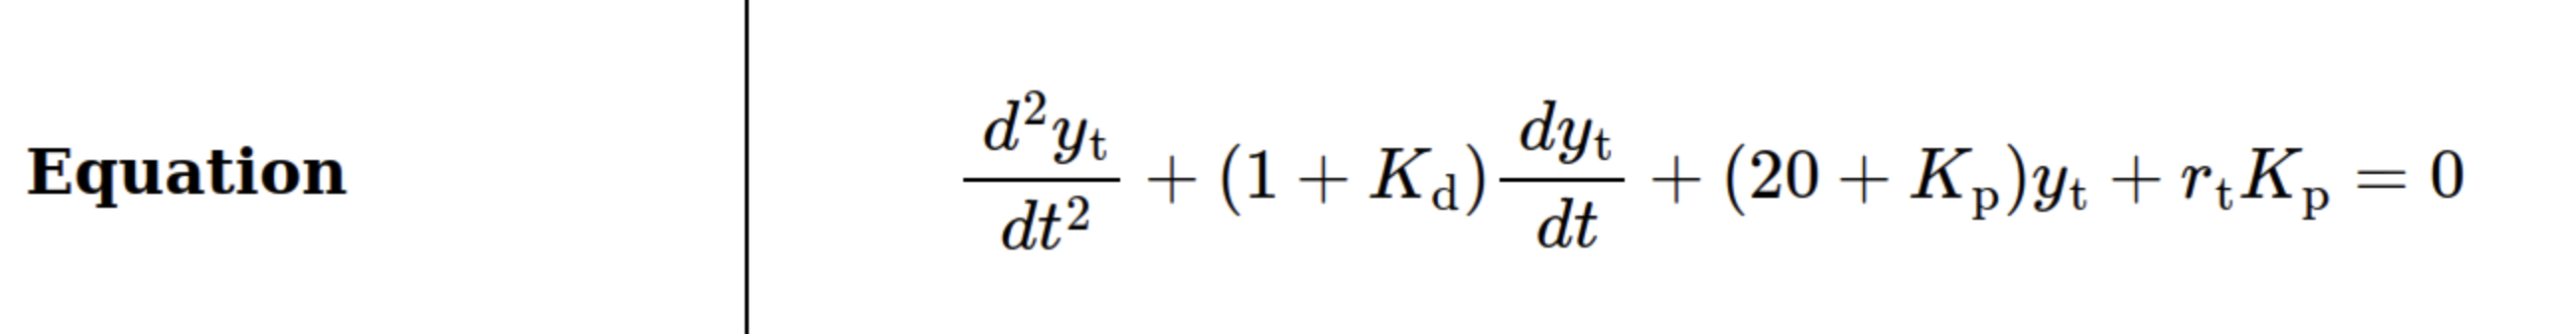
\includegraphics[width=1\textwidth]{figures/ODEVariousForm.png}
\caption{Options of Displaying an ODE}
\label{fig_odevariousform}
\end{figure}
This is just one example of the variability of displaying ODEs. More research is still needed to allow Drasil to display ODEs in various forms.

\section{Allow Adaptive Steps}
While we were solving the ODE as an IVP numerically, we set the step size to a fixed step size. In reality, the step size can be adaptive rather than fixed. We can solve with an adaptive solver and still output the results at a fixed step size. We found some algorithms use a fixed step size for calculating numerical solutions, and others use an adaptive step size. We add the step size with the current time value to calculate the next value of dependent variables. A fixed step size means the step size is the same in each iteration. An adaptive step size means the step size is not always the same and could change based on other factors. In Table~\ref{tab_algacm}, the ACM library divides algorithms into one group that uses a fixed step and others that uses an adaptive step. This discovery can further influence the design choice of solving ODE numerically in the Drasil framework. Currently, Drasil treats all step sizes as a fixed value, and it would be ideal to allow the step size to be either fixed or adaptive in the future.

\section{Solve ODEs as a BVP}
Currently, we solve ODEs as an IVP in Drasil. Solving the ODE as a BVP is another option. The starting point could be to find a suitable external library that can solve the ODE as a BVP. Then, we can generate code to link with this library. Lastly, the input of initial conditions was designed for IVPs, so a new design is required to accept both initial values and boundary values.

\section{Handle Dependency}
Once the Drasil framework generates code, the generated code relies on external libraries to calculate an ODE. In the current setting, the Drasil framework keeps copies of external libraries in the repository. In the long run, this is not practical because of the amount of space external libraries occupy. Moreover, external libraries are not currently shared across case studies, and each case study will have its own copy of external libraries. The current research has uncovered that the current way of handling dependencies in the Drasil framework is problematic. In the future, the team would like to find a better way to handle dependencies. We used a temporary solution, symbolic links, to share external libraries without duplications. By creating a symbolic link file, external libraries become sharable. In the future, the team will conduct further studies to tackle this problem more elegantly.

\section{Define ODE Solver in Drasil}
Our ultimate goal is to write the ODE solver in the Drasil language. Currently, the ODE solver is four selected external libraries. They help us to produce a numerical solution. In future, we want to remove all external libraries and design Drasil's ODE solvers to solve ODEs. Capturing the full knowledge of ODE solvers will take considerable time, but the generated code may be able to take advantage of problem-specified parameters to achieve efficiency not possible with general purpose code.
                  
    \setcounter{figure}{0}
    \setcounter{equation}{0}
    \setcounter{table}{0}

  % \chapter{Your Chapter Title}

This is a sample chapter

If you need to use quotes, type it ``like this''.

\section{Referencing}
These are some sample references to GAMYGDALA~\citep{popescu2014gamygdala} from 
the \texttt{references.bib} file and state effects of 
cognition~\citep{hudlicka2002time} from the \texttt{references\_another.bib} 
file. These references are not in the same .bib file.

\section{Figures}
This is a single image figure (Figure~\ref{fig_singleenv}):

\begin{figure}[ht]
    \centering
    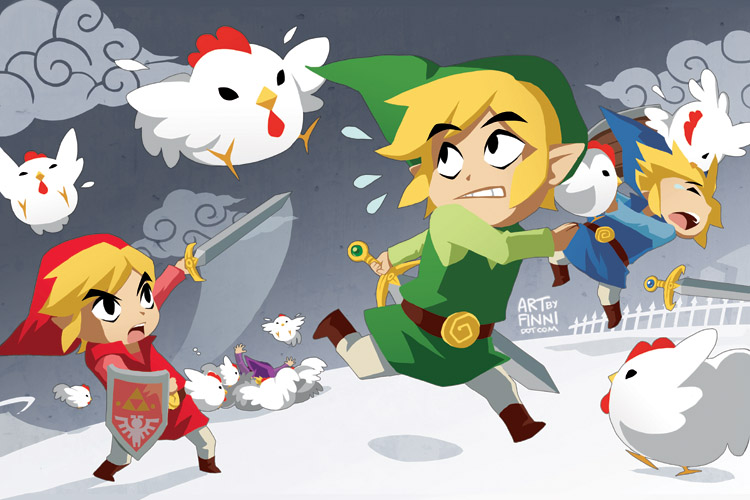
\includegraphics[width=0.6\textwidth]{figures/Sample/tumblr_static_eaceks0rfxsss8o4swscw40wo.jpg}
    \caption[Single Figure Environment Listed Title]{This is a single figure 
    environment}
    \label{fig_singleenv}
\end{figure}

This is a multi-image figure with a top (Figure~\ref{fig_multienv_1}) and bottom (Figure~\ref{fig_multienv_2}) aligned subfigures:

\begin{figure}[ht]
	\centering
	\begin{subfigure}[t]{\textwidth}
		\centering
		
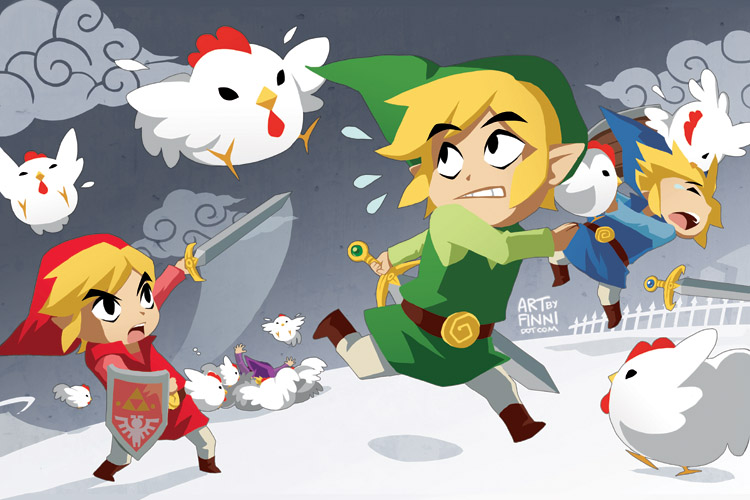
\includegraphics[width=0.7\textwidth]{figures/Sample/tumblr_static_eaceks0rfxsss8o4swscw40wo.jpg}
		\caption{Figure 1}
		\label{fig_multienv_1}
	\end{subfigure}
	~
	\begin{subfigure}[t]{\textwidth}
		\centering
		
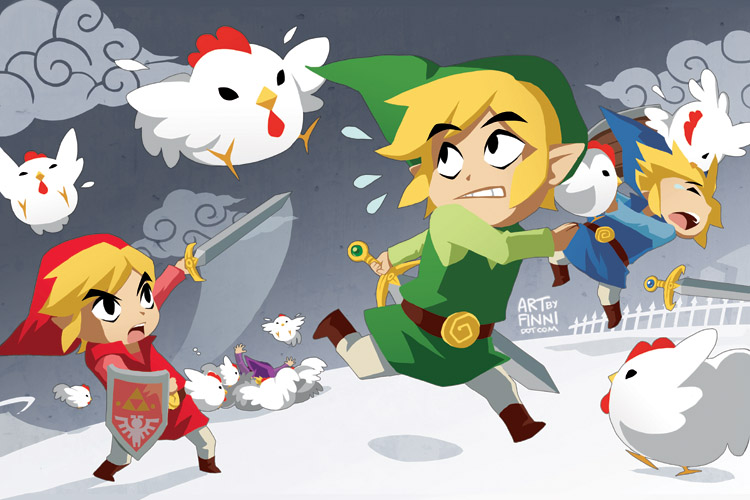
\includegraphics[width=0.7\textwidth]{figures/Sample/tumblr_static_eaceks0rfxsss8o4swscw40wo.jpg}
		\caption{Figure 2}
		\label{fig_multienv_2}
	\end{subfigure}
	
	\caption{A Multi-Figure Environment}
	\label{fig_multienv}
\end{figure}

\section{Tables}

Here is a sample table (Table~\ref{tab_sample}):

	\begin{table}[ht]
	\centering
	\begin{tabular}{ m{0.2\textwidth} m {0.1\textwidth} m{0.15\textwidth} }
		\toprule
		A & $\longleftrightarrow$ & B \\
		C & $\longleftrightarrow$ & D \\
		\bottomrule	
	\end{tabular}	
	\caption{A sample table}	
	\label{tab_sample}
\end{table}

\subsection{Long Tables}
A sample long table is shown in Appendix~\ref{appendix_b}.

\section{Equations}

Here is a sample equation (Equation~\ref{eq_lineslope}):

\begin{equation} \label{eq_lineslope}
	y = mx + b
\end{equation}                  
  %   \setcounter{figure}{0}
  %   \setcounter{equation}{0}
  %   \setcounter{table}{0}

  \chapter{Conclusion}
An ODE is a type, and it exists in many forms. Previously to this research, the Drasil Framework had no flexible and reusable structure for capturing ODE information. The Drasil teams have to manually extract useful information from the original ODE to instruct the Drasil Code Generator to generate code. This approach propagates duplicated information and loses traceability. The newly created structure, \verb|DifferentialModel|, stores linear ODE information based on the conventional matrix concept. It provides the flexibility to transform a linear ODE from one form to another mathematically equivalent form. Once we capture the knowledge of ODE in the new structure, we can reuse it for other purposes, such as producing the numerical solution and displaying the ODE.

Along with \verb|DifferentialModel|, four selected external libraries are responsible for producing the numerical solution for a system of first-order ODEs. Drasil users can get a numerical solution by choosing an algorithm. Currently, although the Calculations module outputs a finite stream of real numbers, $\mathbb{R}^m$, there are other design options. The C\# OSLO provides an option to output an infinite stream of real numbers, $\mathbb{R}^{\infty}$. It has richer data than $\mathbb{R}^m$. Also, outputting the ODE as a function that can return the value of the dependent variable for any value of the independent variable could help generate libraries in Drasil. We did not complete implementing the new specifications for this, but the analysis provides a starting point for future research.

\verb|DifferentialModel| provides reusable ODE information, and external libraries provide mathematical knowledge for solving the ODE. Before we bridge the gap between \verb|DifferentialModel| and external libraries, we enable solving any higher-order ODEs with manually written equations via external libraries. The Double Pendulum case study demonstrates the Drasil Framework can generate code that solves a system of higher-order nonlinear ODEs. With all implementations, we are ready to bridge the gap by automating the process of extracting useful information from \verb|DifferentialModel| and then forming an \verb|ODEInfo|. While we are solving a single higher-order linear ODE, we generate the \verb|ODEInfo| instead of manually creating it. The automation removes the duplicated information and potentially increases traceability.

This research accomplishes three main goals. Firstly, we capture the knowledge of linear ODE in a flexible and reusable structure. Secondly, we expand the Drasil capability to solve any higher-order ODEs with manually written equations. The last one is removing the duplicated information caused by the implementation of solving ODEs.

    \setcounter{figure}{0}
    \setcounter{equation}{0}
    \setcounter{table}{0}

\begin{appendix}
    \chapter{My Appendix}
\label{appendix_a}

This appendix lists tables and code to further explain some parts of this report.

\section{Constructors of DifferentialModel}
\label{const_de}

% \begin{listing}[ht]
\begin{haskell1}
-- $K_d$ is qdDerivGain
-- $y_t$ is opProcessVariable
-- $K_p$ is qdPropGain
-- $r_t$ is qdSetPointTD
imPDRC :: DifferentialModel
imPDRC = makeASingleDE
	time
	opProcessVariable
	lhs
	rhs
	"imPDRC"
	(nounPhraseSP "Computation of the Process Variable as a function of time")
	EmptyS
	where 
	lhs = [exactDbl 1 `addRe` sy qdDerivGain $* (opProcessVariable $^^ 1)]
	$+ (exactDbl 1 $* (opProcessVariable $^^ 2))
	$+ (exactDbl 20 `addRe` sy qdPropGain $* (opProcessVariable $^^ 0))
	rhs = sy qdSetPointTD `mulRe` sy qdPropGain
\end{haskell1}
\captionof{listing}{Using Input Language for the Example~\ref{eq_odeexmaple} in DifferentialModel}
% \label{code_scexinputl}
% \end{listing}

% \begin{listing}[ht]
% \begin{haskell1}
% imPDRC :: DifferentialModel
% imPDRC = makeASystemDE
% 	time
% 	opProcessVariable
% 	coeffs = [[exactDbl 1, exactDbl 1 `addRe` sy qdDerivGain, exactDbl 20 `addRe` sy qdPropGain]]
% 	unknowns = [2, 1, 0]
% 	constants = [sy qdSetPointTD `mulRe` sy qdPropGain]
% 	"imPDRC"
% 	(nounPhraseSP "Computation of the Process Variable as a function of time")
% 	EmptyS
% \end{haskell1}
% \captionof{listing}{Explicitly set values for the example~\ref{eq_odeexmaple} in DifferentialModel}
% \label{code_scexmatrix}
% \end{listing}

\pagebreak

\section{Numerical Solution Implementation}
\label{numsol}

% \begin{listing}[ht]
\begin{python1}
def func_y_t(K_d, K_p, r_t, t_sim, t_step):
    def f(t, y_t):
        return [y_t[1], -(1.0 + K_d) * y_t[1] + -(20.0 + K_p) * y_t[0] + r_t * K_p]
    
    r = scipy.integrate.ode(f)
    r.set_integrator("dopri5", atol=Constants.Constants.AbsTol, rtol=Constants.Constants.RelTol)
    r.set_initial_value([0.0, 0.0], 0.0)
    y_t = [[0.0, 0.0][0]]
    while r.successful() and r.t < t_sim:
        r.integrate(r.t + t_step)
        y_t.append(r.y[0])
    
    return y_t
\end{python1}
\captionof{listing}{Source Code of Solving PDController in Scipy}
% \label{code_pythonscipy}
% \end{listing}

% \begin{listing}[ht]
\begin{java1}
public static ArrayList<Double> func_y_t(double K_d, double K_p, double r_t, double t_sim, double t_step) {
	ArrayList<Double> y_t;
	ODEStepHandler stepHandler = new ODEStepHandler();
	ODE ode = new ODE(K_p, K_d, r_t);
	double[] curr_vals = {0.0, 0.0};

	FirstOrderIntegrator it = new DormandPrince54Integrator(t_step, t_step, Constants.AbsTol, Constants.RelTol);
	it.addStepHandler(stepHandler);
	it.integrate(ode, 0.0, curr_vals, t_sim, curr_vals);
	y_t = stepHandler.y_t;

	return y_t;
}
\end{java1}
\captionof{listing}{A Linear System of First-order Representation in ACM}
% \label{code_javaacm}
% \end{listing}

% \begin{listing}
\begin{cplusplus1}
vector<double> func_y_t(double K_d, double K_p, double r_t, double t_sim, double t_step) {
	vector<double> y_t;
	ODE ode = ODE(K_p, K_d, r_t);
	vector<double> currVals{0.0, 0.0};
	Populate pop = Populate(y_t);
		
	boost::numeric::odeint::runge_kutta_dopri5<vector<double>> rk = boost::numeric::odeint::runge_kutta_dopri5<vector<double>>();
	auto stepper = boost::numeric::odeint::make_controlled(Constants::AbsTol, Constants::RelTol, rk);
	boost::numeric::odeint::integrate_const(stepper, ode, currVals, 0.0, t_sim, t_step, pop);
	
	return y_t;
}	
\end{cplusplus1}
\captionof{listing}{A Linear System of First-order Representation in ODEINT}
% \label{code_cplusplusodeint}
% \end{listing}

% \begin{listing}[ht]
% \begin{csharp1}
% public static List<double> func_y_t(double K_d, double K_p, double r_t, double t_sim, double t_step) {
% 	List<double> y_t;
% 	Func<double, Vector, Vector> f = (t, y_t_vec) => {
% 		return new Vector(y_t_vec[1], -(1.0 + K_d) * y_t_vec[1] + -(20.0 + K_p) * y_t_vec[0] + r_t * K_p);
% 	};
% 	Options opts = new Options();
% 	opts.AbsoluteTolerance = Constants.AbsTol;
% 	opts.RelativeTolerance = Constants.RelTol;
	
% 	Vector initv = new Vector(new double[] {0.0, 0.0});
% 	IEnumerable<SolPoint> sol = Ode.RK547M(0.0, initv, f, opts);
% 	IEnumerable<SolPoint> points = sol.SolveFromToStep(0.0, t_sim, t_step);
% 	y_t = new List<double> {};
% 	foreach (SolPoint sp in points) {
% 		y_t.Add(sp.X[0]);
% 	}
	
% 	return y_t;
% }
% \end{csharp1}
% \captionof{listing}{Source code of solving PDController in OSLO}
% \label{code_csharposlo}
% \end{listing}

\pagebreak

\section{Algorithm in External Libraries}
\label{alg_externallib}

\begin{table}[ht]
\begin{tabular}{ p{0.2\textwidth} p{0.7\textwidth} }
	\textbf{Name} & \textbf{Description} \\
	\toprule
	\verb|zvode| & Complex-valued Variable-coefficient Ordinary Differential Equation solver, with fixed-leading-coefficient implementation. It provides implicit Adams method (for non-stiff problems) and a method based on backward differentiation formulas (BDF) (for stiff problems).\\ \hline
	\verb|lsoda| & Real-valued Variable-coefficient Ordinary Differential Equation solver, with fixed-leading-coefficient implementation. It provides automatic method switching between implicit Adams method (for non-stiff problems) and a method based on backward differentiation formulas (BDF) (for stiff problems).\\ \hline
	\verb|dopri5| & This is an explicit runge-kutta method of order (4)5 due to Dormand \& Prince (with stepsize control and dense output).\\ \hline
	\verb|dop853| & This is an explicit runge-kutta method of order 8(5,3) due to Dormand \& Prince (with stepsize control and dense output).\\
	\bottomrule	
\end{tabular}	
\caption{Algorithm Options in Scipy - Python~\citep{scipyfun}}	
\label{tab_algscipy}
\end{table}

\begin{table}[ht]
\begin{tabular}{ p{0.2\textwidth} p{0.7\textwidth} }
	\textbf{Name} & \textbf{Description} \\
	\toprule
	\verb|RK547M| & This method is most appropriate for solving non-stiff ODE systems. It is based on classical Runge-Kutta formulae with modifications for automatic error and step size control.\\ \hline
	\verb|GearBDF| & It is an implementation of the Gear back differentiation method, a multi-step implicit method for stiff ODE systems solving.\\
	\bottomrule	
\end{tabular}	
\caption{Algorithm Options in OSLO - C\#~\citep{oslofun}}	
\label{tab_algodeint}
\end{table}

\begin{table}
\begin{tabular}{ p{0.13\textwidth} | p{0.27\textwidth} p{0.57\textwidth} }
	\textbf{Step Size} & \textbf{Name} & \textbf{Description} \\
	\toprule
	Fixed Step & \verb|Euler| & This class implements a simple Euler integrator for Ordinary Differential Equations.\\ \hline
	& \verb|Midpoint| & This class implements a second order Runge-Kutta integrator for Ordinary Differential Equations.\\ \hline
	& \verb|Classical RungeKutta| & This class implements the classical fourth order Runge-Kutta integrator for Ordinary Differential Equations (it is the most often used Runge-Kutta method).\\ \hline
	& \verb|Gill| & This class implements the Gill fourth order Runge-Kutta integrator for Ordinary Differential Equations.\\ \hline
	& \verb|Luther| & This class implements the Luther sixth order Runge-Kutta integrator for Ordinary Differential Equations.\\ \hline
	Adaptive Stepsize & \verb|Higham and Hall| & This class implements the 5(4) Higham and Hall integrator for Ordinary Differential Equations.\\ \hline
	& \verb|DormandPrince 5(4)| & This class implements the 5(4) Dormand-Prince integrator for Ordinary Differential Equations.\\ \hline
	& \verb|DormandPrince 8(5,3)| & This class implements the 8(5,3) Dormand-Prince integrator for Ordinary Differential Equations.\\ \hline
	& \verb|Gragg-Bulirsch-Stoer| & This class implements a Gragg-Bulirsch-Stoer integrator for Ordinary Differential Equations.\\ \hline
	& \verb|Adams-Bashforth| & This class implements explicit Adams-Bashforth integrators for Ordinary Differential Equations.\\ \hline
	& \verb|Adams-Moulton| & This class implements implicit Adams-Moulton integrators for Ordinary Differential Equations.\\
	\bottomrule	
\end{tabular}	
\caption{Algorithm Options in Apache Commons Maths - Java~\citep{apachefun}}	
\label{tab_algacm}
\end{table}

\begin{table}
\begin{tabular}{ p{0.4\textwidth} p{0.5\textwidth} }
	\textbf{Name} & \textbf{Description} \\
	\toprule
	\verb|euler| & Explicit Euler: Very simple, only for demonstrating purpose\\ \hline
	\verb|runge_kutta4| & Runge-Kutta 4: The classical Runge Kutta scheme, good general scheme without error control.\\ \hline
	\verb|runge_kutta_cash_karp54| & Cash-Karp: Good general scheme with error estimation.\\ \hline
	\verb|runge_kutta_dopri5| & Dormand-Prince 5: Standard method with error control and dense output.\\ \hline
	\verb|runge_kutta_fehlberg78| & Fehlberg 78: Good high order method with error estimation.\\ \hline
	\verb|adams_bashforth_moulton| & Adams-Bashforth-Moulton: Multi-step method with high performance.\\ \hline
	\verb|controlled_runge_kutta| & Controlled Error Stepper: Error control for the Runge-Kutta steppers.\\ \hline
	\verb|dense_output_runge_kutta| & Dense Output Stepper: Dense output for the Runge-Kutta steppers.\\ \hline
	\verb|bulirsch_stoer| & Bulirsch-Stoer: Stepper with step size, order control and dense output. Very good if high precision is required..\\ \hline
	\verb|implicit_euler| & Implicit Euler: Basic implicit routine.\\ \hline
	\verb|rosenbrock4| & Rosenbrock 4: Solver for stiff systems with error control and dense output.\\ \hline
	\verb|symplectic_euler| & Symplectic Euler: Basic symplectic solver for separable Hamiltonian system.\\ \hline
	\verb|symplectic_rkn_sb3a_mclachlan| & Symplectic RKN McLachlan: Symplectic solver for separable Hamiltonian system with order 6.\\
	\bottomrule	
\end{tabular}	
\caption{Algorithm Options in ODEINT - C++~\citep{odeintfun}}	
\label{tab_algodeint}
\end{table}

\pagebreak

\section{Generated Code for Double Pendulum}
\label{gencodedbl}
 
We altered the source code to make it more readable. In Code~\ref{code_pythondbl} and Code~\ref{code_csharpdbl}, lines 2-12 are in one line. In Code~\ref{code_javadbl} and Code~\ref{code_cppdbl}, lines 4-5 are in one line. Lines 9-10 are in one line.
\begin{listing}[ht]
\begin{python1}
def f(t, theta):
	return [
		theta[1],

		(-9.8 * (2.0 * m_1 + m_2) * math.sin(theta[0]) - m_2 * 9.8 * math.sin(theta[0] - 2.0 * theta[2]) - 2.0 * math.sin(theta[0] - theta[2]) * m_2 * (theta[3] ** 2.0 * L_2 + theta[1] ** 2.0 * L_1 * math.cos(theta[0] - theta[2]))) 
			/ (L_1 * (2.0 * m_1 + m_2 - m_2 * math.cos(2.0 * theta[0] - 2.0 * theta[2]))), 
		
		theta[3], 
		
		2.0 * math.sin(theta[0] - theta[2]) * (theta[1] ** 2.0 * L_1 * (m_1 + m_2) + 9.8 * (m_1 + m_2) * math.cos(theta[0]) + theta[3] ** 2.0 * L_2 * m_2 * math.cos(theta[0] - theta[2])) 
			/ (L_2 * (2.0 * m_1 + m_2 - m_2 * math.cos(2.0 * theta[0] - 2.0 * theta[2])))
		]
\end{python1}
\captionof{listing}{Generate Python Code for Double Pendulum}
\label{code_pythondbl}
\end{listing} 

\begin{listing}[ht]
\begin{csharp1}
Func<double, Vector, Vector> f = (t, theta_vec) => {
	return new Vector(
		theta_vec[1], 

		(-9.8 * (2.0 * m_1 + m_2) * Math.Sin(theta_vec[0]) - m_2 * 9.8 * Math.Sin(theta_vec[0] - 2.0 * theta_vec[2]) - 2.0 * Math.Sin(theta_vec[0] - theta_vec[2]) * m_2 * (Math.Pow(theta_vec[3], 2.0) * L_2 + Math.Pow(theta_vec[1], 2.0) * L_1 * Math.Cos(theta_vec[0] - theta_vec[2]))) 
			/ (L_1 * (2.0 * m_1 + m_2 - m_2 * Math.Cos(2.0 * theta_vec[0] - 2.0 * theta_vec[2]))), 
		
		theta_vec[3], 

		2.0 * Math.Sin(theta_vec[0] - theta_vec[2]) * (Math.Pow(theta_vec[1], 2.0) * L_1 * (m_1 + m_2) + 9.8 * (m_1 + m_2) * Math.Cos(theta_vec[0]) + Math.Pow(theta_vec[3], 2.0) * L_2 * m_2 * Math.Cos(theta_vec[0] - theta_vec[2])) 
			/ (L_2 * (2.0 * m_1 + m_2 - m_2 * Math.Cos(2.0 * theta_vec[0] - 2.0 * theta_vec[2]))));
};
\end{csharp1}
\captionof{listing}{Generate C\# Code for Double Pendulum}
\label{code_csharpdbl}
\end{listing} 

\begin{listing}[ht]
\begin{java1}
public void computeDeriv(double t, double[] theta, double[] dtheta) {
	dtheta[0] = theta[1];

	dtheta[1] = (-9.8 * (2.0 * m_1 + m_2) * Math.sin(theta[0]) - m_2 * 9.8 * Math.sin(theta[0] - 2.0 * theta[2]) - 2.0 * Math.sin(theta[0] - theta[2]) * m_2 * (Math.pow(theta[3], 2.0) * L_2 + Math.pow(theta[1], 2.0) * L_1 * Math.cos(theta[0] - theta[2]))) 
		/ (L_1 * (2.0 * m_1 + m_2 - m_2 * Math.cos(2.0 * theta[0] - 2.0 * theta[2])));
	
	dtheta[2] = theta[3];

	dtheta[3] = 2.0 * Math.sin(theta[0] - theta[2]) * (Math.pow(theta[1], 2.0) * L_1 * (m_1 + m_2) + 9.8 * (m_1 + m_2) * Math.cos(theta[0]) + Math.pow(theta[3], 2.0) * L_2 * m_2 * Math.cos(theta[0] - theta[2])) 
		/ (L_2 * (2.0 * m_1 + m_2 - m_2 * Math.cos(2.0 * theta[0] - 2.0 * theta[2])));
}
\end{java1}
\captionof{listing}{Generate Java Code for Double Pendulum}
\label{code_javadbl}
\end{listing}

\begin{listing}[ht]
\begin{cplusplus1}
void ODE::operator()(vector<double> theta, vector<double> &dtheta, double t) {
	dtheta.at(0) = theta.at(1);

	dtheta.at(1) = (-9.8 * (2.0 * m_1 + m_2) * sin(theta.at(0)) - m_2 * 9.8 * sin(theta.at(0) - 2.0 * theta.at(2)) - 2.0 * sin(theta.at(0) - theta.at(2)) * m_2 * (pow(theta.at(3), 2.0) * L_2 + pow(theta.at(1), 2.0) * L_1 * cos(theta.at(0) - theta.at(2)))) 
		/ (L_1 * (2.0 * m_1 + m_2 - m_2 * cos(2.0 * theta.at(0) - 2.0 * theta.at(2))));
	
	dtheta.at(2) = theta.at(3);

	dtheta.at(3) = 2.0 * sin(theta.at(0) - theta.at(2)) * (pow(theta.at(1), 2.0) * L_1 * (m_1 + m_2) + 9.8 * (m_1 + m_2) * cos(theta.at(0)) + pow(theta.at(3), 2.0) * L_2 * m_2 * cos(theta.at(0) - theta.at(2))) 
		/ (L_2 * (2.0 * m_1 + m_2 - m_2 * cos(2.0 * theta.at(0) - 2.0 * theta.at(2))));
}
\end{cplusplus1}
\captionof{listing}{Generate C\texttt{++} Code for Double Pendulum}
\label{code_cppdbl}
\end{listing} 

      \setcounter{figure}{0}
      \setcounter{equation}{0}
      \setcounter{table}{0}

    % \chapter{Long Tables}
\label{appendix_b}

This appendix demonstrates the use of a long table that spans multiple pages.

\begin{center}
\begin{longtable}{P{3cm}P{3cm}P{2.5cm}P{3.5cm}}
\toprule
\hline
\textbf{Col A} & \textbf{Col B} & \textbf{Col C} & \textbf{Col D} \\ \midrule

\endfirsthead
\multicolumn{4}{c}{\textit{Continued from previous page}} \\ \hline
\textbf{Col A} & \textbf{Col B} & \textbf{Col C} & \textbf{Col D} \\ \hline
\endhead
\hline \multicolumn{4}{r}{\textit{Continued on the next page}} \\
\endfoot
\hline
\endlastfoot

A & B & C & D \\ \midrule

A & B & C & D \\ \midrule

A & B & C & D \\ \midrule

A & B & C & D \\ \midrule

A & B & C & D \\ \midrule

A & B & C & D \\ \midrule

A & B & C & D \\ \midrule

A & B & C & D \\ \midrule

A & B & C & D \\ \midrule

A & B & C & D \\ \midrule

A & B & C & D \\ \midrule

A & B & C & D \\ \midrule

A & B & C & D \\ \midrule

A & B & C & D \\ \midrule

A & B & C & D \\ \midrule

A & B & C & D \\ \midrule

A & B & C & D \\ \midrule

A & B & C & D \\ \midrule

A & B & C & D \\ \midrule

A & B & C & D \\ \midrule

\hline
\end{longtable}
\end{center}

    %   \setcounter{figure}{0}
    %   \setcounter{equation}{0}
    %   \setcounter{table}{0}

\end{appendix}

% The bibliography is set up to allow for multiple bib files
\bibliographystyle{acm}
\bibliography{references}
% \bibliography{references,references_another}

\label{NumDocumentPages}

\end{document}
% ********************************
